% !TEX root = ../OT4ML.tex

%%%%%%%%%%%%%%%%%%%%%%%%%%%%%%%%%%%%%%%%%%%%%%%%%%%%%%%%%%%%%%%%%%%%%%%%%%%
%%%%%%%%%%%%%%%%%%%%%%%%%%%%%%%%%%%%%%%%%%%%%%%%%%%%%%%%%%%%%%%%%%%%%%%%%%%
%%%%%%%%%%%%%%%%%%%%%%%%%%%%%%%%%%%%%%%%%%%%%%%%%%%%%%%%%%%%%%%%%%%%%%%%%%%
\chapter{Monge Problem between Measures}
\index{Monge!problem}% strictindex
\label{sec-monge}

The goal of this chapter is to pass from finite matching to transport between arbitrary probability laws. The central stakes are to define measures, push-forwards and Monge maps carefully enough that the discrete picture survives, while exposing why deterministic maps can fail to exist. Monge's original formulation~\cite{Monge1781} and modern treatments~\cite{Villani03,Villani09,SantambrogioBook,rachev1998mass} are the conceptual background for this transition.
\index{push-forward}% strictindex
\index{Monge!map}% strictindex

The strict assignment model of the previous chapter handles uniform point clouds of equal cardinality. Passing to arbitrary measures allows unequal weights, continuous densities and singular distributions to be treated within one language.

%%%%%%%%%%%%%%%%%%%%%%%%%%%%%%%%%%%%%%%%%%%%%%%%%%%%%%%%%%%%%%%%%%%%%%%%%%%
\section{Measures}
\label{sec-measures}

Measures are the language that lets point clouds, densities and singular objects be handled uniformly. We only recall the facts needed later: integration, total variation, densities and probabilistic laws.
\index{total variation}% strictindex

\paragraph{Histograms}
\index{histogram}% strictindex

The finite-dimensional model for a probability law is a nonnegative vector with unit total mass.

\begin{defn}[Probability simplex]\label{def-probability-simplex}
\index{probability simplex}% strictindex
	The probability simplex of length $n$ is
	\[
		\simplex_n \eqdef \enscond{\a \in \RR_+^n}{ \sum_{i=1}^n \a_i = 1 }.
	\]
	Its elements are also called probability vectors or histograms.
\end{defn}

\paragraph{Discrete measure, empirical measure}
\index{discrete!measure}% strictindex
\index{empirical!measure}% strictindex

Probability vectors become measures once their masses are attached to locations.

\begin{defn}[Discrete measure]\label{def-discrete-measure}
\index{Dirac mass}% strictindex
	A discrete measure with weights $\a$ and locations $x_1,\dots,x_n\in\X$ is
	\eql{\label{eq-discr-meas}
			\al = \sum_{i=1}^n \a_i \de_{x_i},
	}
	where $\de_x$ is the Dirac mass at position $x$. It is a probability measure if $\a\in\simplex_n$, and a positive measure if all weights $\a_i$ are nonnegative.
\end{defn}
The Dirac mass should be thought of as a unit of mass infinitely concentrated at one location.
\index{probability measure}% strictindex
\index{Dirac mass}% strictindex
%
The empirical probability distribution of a point cloud is $\al=\frac{1}{n}\sum_i \de_{x_i}$.
%
Many applications manipulate both the positions $x_i$ (a Lagrangian discretization) and the weights $\a_i$ (an Eulerian discretization). Moving the positions gives an adaptive representation, but usually destroys convexity; changing only the weights often preserves it.


%%%%
\paragraph{General measures}

We consider finite signed Borel measures $\al \in \Mm(\X)$ on a metric space $(\Xx,d)$. The Borel sets form the smallest $\sigma$-algebra containing all open subsets of $\Xx$, obtained by closing the open sets under complements and countable unions. Unless otherwise stated, all measures are finite.
\index{Borel set}% strictindex
\index{Borel measure}% strictindex
%
A Dirac measure $\de_x$ is then defined as $\de_x(A)=1$ if $x \in A$ and $0$ otherwise, and this extends by linearity for discrete measures of the form~\eqref{eq-discr-meas} as
\index{Dirac mass}% strictindex
\eq{
	\al(A) = \sum_{x_i \in A} \a_i
}
%
Positive and probability measures are formalized below together with the Radon regularity used throughout the book.

\paragraph{Polish metric spaces.}
\index{Polish space}% strictindex
Many measure-theoretic statements used later require a mild regularity assumption on the underlying space. The point is not to restrict applications, since Euclidean spaces, complete separable manifolds and separable Hilbert spaces are covered, but to exclude pathological measurable spaces where disintegration, tightness or weak convergence can fail to behave properly.
\index{metric!space}% strictindex
\index{weak!convergence}% strictindex
\index{tightness}% strictindex

\begin{defn}[Polish metric space]\label{def-polish-metric-space}
	A metric space $(\X,d)$ is Polish if it is complete and separable: every Cauchy sequence converges in $\X$, and $\X$ contains a countable dense subset. More generally, a topological space is called Polish if its topology can be induced by some complete separable metric.
\index{complete metric space}% strictindex
\index{separable space}% strictindex
\index{countable dense subset}% strictindex
\end{defn}
This assumption already includes genuinely infinite-dimensional spaces. In the Euclidean dynamic OT and Schr\"odinger formulations of Sections~\ref{rem-bb-path-space} and~\ref{sec-path-space-schrodinger}, the path space
\eq{
	\Ss=C([0,1];\RR^d),\qquad
	d_\infty(\gamma,\eta) \eqdef \sup_{t\in[0,1]}\norm{\gamma(t)-\eta(t)}
}
is Polish. Completeness follows because a uniformly Cauchy sequence of continuous paths converges uniformly to a continuous path, and separability follows by approximating paths uniformly by piecewise-linear paths with rational breakpoints and rational values. This path space supports laws of trajectories: its endpoint evaluation maps are continuous, which makes endpoint constraints well behaved for dynamical optimal plans and Schr\"odinger bridges.
\index{path space}% strictindex
\index{continuous!path}% strictindex
Polish spaces are the natural ambient category for probability measures. Borel probability measures on them are regular, tightness gives compactness criteria, regular conditional probabilities and disintegrations exist under standard assumptions, and Wasserstein spaces remain Polish; see Proposition~\ref{prop-wasserstein-space-polish}.
\index{probability measure}% strictindex
\index{Borel measure}% strictindex
\index{conditional!probability}% strictindex
\index{disintegration}% strictindex

\begin{defn}[Support of a measure]\label{def:support}
\index{support}% strictindex
	Let $\al$ be a positive Borel measure on a metric space $\Xx$. Its support is
	\[
		\supp(\al)
		\eqdef
		\enscond{x\in\Xx}{\al(B(x,r))>0\text{ for every }r>0}.
	\]
	If $\Xx$ is separable, this is the smallest closed set of full $\al$-mass.
\end{defn}


%%%%
\paragraph{Radon measures}
\index{Radon measure}% strictindex

Radon regularity ensures that Borel measures can be approximated from within by compact sets and paired reliably with test functions.
\index{Borel set}% strictindex
\index{measurable function}% strictindex
\index{Borel measure}% strictindex
\begin{defn}[Radon and probability measures]\label{def-radon-probability-measures}
	A locally finite positive Borel measure $\al$ on $\Xx$ is Radon if
	\[
		\al(A)=\sup\enscond{\al(K)}{K\subset A\text{ compact}}
	\]
	for every Borel set $A$. We write $\Mm_+(\Xx)$ for finite positive Radon measures and
	$\Mm_+^1(\Xx)=\enscond{\al\in\Mm_+(\Xx)}{\al(\Xx)=1}$ for probability measures.
\end{defn}
Every finite Borel measure on a Polish space is Radon.
\index{probability measure}% strictindex
For an integrable function $f$, we use the pairing notation
\[
	\dotp{f}{\al}\eqdef\int_\Xx f(x)\d\al(x).
\]
Integration of such a measurable $f$ against a discrete measure $\al$ computes a sum
\eq{
	\int_\X f(x) \d\al(x) = \sum_{i=1}^n \a_i f(x_i).
}


This applies in particular to continuous test functions, which are Borel measurable.
%
Integration against a finite measure on a compact space thus defines a continuous linear form $f \mapsto \int f \d\al$ on the Banach space of continuous functions $(\Cc(\Xx),\norm{\cdot}_\infty)$, indeed $|\int f \d\al| \leq \norm{f}_\infty |\al|(\Xx)$. On compact spaces, the converse is true: every continuous linear form on $\Cc(\Xx)$ is represented by integration against a finite signed Radon measure. This is the Riesz--Markov--Kakutani representation theorem~\cite{rudin1987realcomplex,bogachev2007measure}. It identifies $\Mm(\Xx)$ with the Banach dual of $\Cc(\Xx)$, and this duality pairing $\dotp{f}{\al}$ will be crucial for the convex duality arguments used later.
\index{Radon measure}% strictindex
\index{Banach space}% strictindex
\index{Banach dual}% strictindex
\index{linear!form}% strictindex
\index{finite measure}% strictindex
\index{Riesz-Markov-Kakutani theorem}% strictindex
\index{dual!pairing}% strictindex

%%%%%
\paragraph{Relative densities.}
\index{density!ratio}% strictindex

Many formulas below compare measures through densities with respect to a reference measure.

\begin{defn}[Relative density]\label{def-relative-density}
\index{Lebesgue measure}% strictindex
\index{reference!measure}% strictindex
\index{density!relative}% strictindex
	If $\al$ is absolutely continuous with respect to a positive reference measure $\lambda$, its relative density is the Radon--Nikodym derivative
	\[
		\density{\al}\eqdef\frac{\d\al}{\d\lambda},
		\qquad
		\d\al(x)=\density{\al}(x)\d\lambda(x).
	\]
	Equivalently, for every bounded measurable function $h$, and more generally whenever $h$ is integrable with respect to the total variation of $\al$,
	\[
		\int_{\Xx} h(x) \d\al(x) = \int_{\Xx} h(x) \density{\al}(x) \d\lambda(x).
	\]
	If $\al$ is positive, the same identity holds in $[0,+\infty]$ for every nonnegative measurable $h$.
\end{defn}
On $\RR^d$ the reference $\lambda$ is often Lebesgue measure $\d x$.

%%%%%
\paragraph{Total variation norm.}
\index{total variation}% strictindex

The norm inherited from the duality $\Mm(\Xx)=\Cc(\Xx)^*$ is the total variation norm. We use the notation
\begin{defn}[Total variation]\label{defn-total-variation}
	For a finite signed Radon measure $\al$ on a compact space $\Xx$,
\index{Radon measure}% strictindex
	\[
		\norm{\al}_{\TV}
		\eqdef
		\usup{f \in \Cc(\Xx)} \enscond{\dotp{f}{\al}}{\norm{f}_\infty \leq 1}.
	\]
\end{defn}
This formula is useful because it computes the norm of a measure as the operator norm of the corresponding linear form on $\Cc(\Xx)$.
\index{linear!form}% strictindex
\index{operator norm}% strictindex

The same norm also has a direct measure-theoretic expression. The absolute value of a signed measure is
\index{signed!measure}% strictindex
\[
	|\al|(A)
	\eqdef
	\usup{A=\cup_i B_i} \sum_i |\al(B_i)|,
\]
where the supremum is over finite or countable measurable partitions of $A$. Thus, if $\al=\sum_i \a_i \de_{x_i}$ with distinct atoms, $|\al|=\sum_i |\a_i|\de_{x_i}$; if $\d\al(x)=\rho(x)\d\lambda(x)$, then $\d|\al|(x)=|\rho(x)|\d\lambda(x)$.

\begin{prop}[Dual and measure definitions of total variation]\label{prop-tv-dual-measure}
\index{total variation}% strictindex
	For a finite signed Radon measure $\al$ on a compact space $\Xx$,
\index{Radon measure}% strictindex
	one has $\norm{\al}_{\TV}=|\al|(\Xx)$.
	Consequently $(\Mm(\Xx),\norm{\cdot}_{\TV})$ is isometrically the Banach dual of $(\Cc(\Xx),\norm{\cdot}_\infty)$.
\index{Banach dual}% strictindex
\end{prop}
\begin{proof}
	The inequality $\norm{\al}_{\TV}\leq |\al|(\Xx)$ follows from
	\[
		\abs{\int f\,\d\al}\leq \int |f|\,\d|\al|\leq \norm{f}_\infty |\al|(\Xx).
	\]
	For the reverse inequality, write the Jordan decomposition $\al=\al^+-\al^-$, so that $|\al|=\al^++\al^-$. The measurable sign $s=\frac{\d\al}{\d|\al|}$ takes values in $\{-1,1\}$ outside a $|\al|$-null set and satisfies $\d\al=s\,\d|\al|$. By regularity of Radon measures on compact spaces, $s$ can be approximated in $L^1(|\al|)$ by continuous functions $f_k$ with $\norm{f_k}_\infty\leq1$. Hence $\int f_k\,\d\al\to\int s\,\d\al=|\al|(\Xx)$, which proves the equality. The final statement is the Riesz--Markov--Kakutani representation theorem with this norm.
\index{Riesz-Markov-Kakutani theorem}% strictindex
\index{Jordan decomposition}% strictindex
\index{Radon measure}% strictindex
\end{proof}

For two absolutely continuous measures $\d\al=\density{\al}\d\lambda$ and $\d\be=\density{\be}\d\lambda$, this gives the concrete formula
\[
	\norm{\al-\be}_{\TV}
	=
	\int_\Xx |\density{\al}(x)-\density{\be}(x)|\,\d\lambda(x).
\]
For two discrete measures, one first recasts both measures as weight vectors on
the same finite support. If
\[
	\al=\sum_{i=1}^n \tilde a_i\delta_{x_i},
	\qquad
	\be=\sum_{j=1}^m \tilde b_j\delta_{y_j},
\]
let $z_1,\ldots,z_r$ be the distinct points in the union
$\{x_i\}_i\cup\{y_j\}_j$ and set
\[
	a_k\eqdef\sum_{i:x_i=z_k}\tilde a_i,
	\qquad
	b_k\eqdef\sum_{j:y_j=z_k}\tilde b_j.
\]
Then $\al=\sum_{k=1}^r a_k\delta_{z_k}$ and
$\be=\sum_{k=1}^r b_k\delta_{z_k}$.
This convention merges masses located at the same point before comparing the two
measures. If the two input supports are already enumerated without repetitions
and are disjoint, this simply amounts to taking
$(z_k)_k=(x_1,\ldots,x_n,y_1,\ldots,y_m)$ and padding the weights as
$a=(\tilde a,0_m)$ and $b=(0_n,\tilde b)$. With this common-support notation,
\[
	\norm{\al-\be}_{\TV}
	=
	\sum_{k=1}^r |a_k-b_k|.
\]
%%%%%
\paragraph{Probabilistic interpretation.}
\index{probabilistic coupling}% strictindex

Probability measures represent random observations through their laws.
\index{random variable}% strictindex
\index{probability measure}% strictindex
\begin{defn}[Random variable and law]\label{def-random-variable-law}
	Let $(\Omega,\Ff,\PP)$ be a probability space and let $\Xx$ be Polish. An $\Xx$-valued random variable is a measurable map $X:(\Omega,\Ff)\to(\Xx,\Bb(\Xx))$. Its law is
	\[
		\operatorname{Law}(X)\eqdef X_\sharp\PP,
		\qquad
		\operatorname{Law}(X)(A)=\PP(X\in A)
	\]
	for every Borel set $A\subset\Xx$.
\end{defn}
\index{Borel set}% strictindex
For every integrable function $f$, integration with respect to this law is expectation:
\[
	\int_\X f(x)\,\d\operatorname{Law}(X)(x)=\EE[f(X)].
\]


%%%%%%%%%%%%%%%%%%%%%%%%%%%%%%%%%%%%%%%%%%%%%%%%%%%%%%%%%%%%%%%%%%%%%%%%%%%
\section{Push-Forward}
\index{push-forward}% strictindex
\label{sec-push-forward}


Push-forwards encode how maps move mass. This short section is the bridge between deterministic maps and linear operations on measures.

For a measurable map $\T : \X \rightarrow \Y$, the push-forward operator $\T_\sharp : \Mm(\X) \rightarrow \Mm(\Y)$ records the distribution of the image points.
%
For a Dirac mass, one has $\T_\sharp \de_{x} = \de_{\T(x)}$. The operation $\al\mapsto\T_\sharp\al$ is linear in the measure, although its definition for a general measure uses inverse images rather than a decomposition into Dirac masses. In this sense, moving from $\T$ to $\T_\sharp$ linearizes the action of a map at the price of passing from a possibly finite-dimensional space $\Xx$ to the infinite-dimensional space $\Mm(\Xx)$, an idea that underlies many convex relaxations.
\index{Dirac mass}% strictindex
%
For discrete measures~\eqref{eq-discr-meas}, the push-forward operation consists simply in moving the positions of all the points in the support of the measure
\index{support}% strictindex
\eq{
	\T_{\sharp} \al \eqdef \sum_i \a_i \de_{\T(x_i)}.
}
For more general measures, for instance for those with a density, the notion of push-forward plays a fundamental role in describing spatial modifications of probability measures. The formal definition reads as follows.
\index{probability measure}% strictindex
\index{push-forward}% strictindex

\begin{defn}[Push-forward]\label{defn-pushfwd}
For a measurable map $\T : \X \rightarrow \Y$ and $\al \in \Mm(\X)$, the push-forward measure $\be = \T_\sharp \al \in \Mm(\Y)$ is defined, for every measurable set $B\subset\Y$, by
\eql{\label{eq-equiv-pushfwd}
	\be(B) = \al\bigl(\enscond{x \in \X}{\T(x) \in B}\bigr).
}
Equivalently, for every bounded measurable function $h:\Y\to\RR$,
\eql{\label{eq-push-fwd}
	\int_\Y h(y) \d \be(y) = \int_\X h(\T(x)) \d\al(x).
}
Note that $\T_\sharp$ preserves positivity and total mass, so that if $\al \in \Mm_+^1(\X)$ then $\T_\sharp \al \in \Mm_+^1(\Y)$.
\end{defn}


\begin{rem}[Pullback and push-forward]\label{rem-pullback-pushforward}\label{rem-push-forward-pull-back}
\index{pullback}% strictindex
\index{push-forward}% strictindex
	Assume that $\X$ and $\Y$ are compact and that $\T:\X\to\Y$ is continuous. The pullback by $\T$ is the bounded linear operator
	\[
		\T^\sharp:\Cc(\Y)\to\Cc(\X),
		\qquad
		\T^\sharp g=g\circ\T.
	\]
	The definition of the push-forward is exactly the dual relation between this pullback on functions and the action of $\T_\sharp$ on measures:
\index{pullback}% strictindex
\index{push-forward}% strictindex
	\[
		\int_\X \T^\sharp g(x)\d\al(x)
		=
		\int_\Y g(y)\d(\T_\sharp\al)(y).
	\]
	In pairing notation,
	\[
		\left\langle \T^\sharp g,\al\right\rangle_{\Cc(\X),\Mm(\X)}
		=
		\left\langle g,\T_\sharp\al\right\rangle_{\Cc(\Y),\Mm(\Y)}.
	\]
	Thus, under the Riesz identification of measures with the duals of continuous functions on compact spaces, push-forward is the Banach adjoint of pullback, with the direction reversed. On noncompact spaces, Equation~\eqref{eq-push-fwd} still gives the same dual relation for bounded measurable test functions, but no such identification with the full dual of $\Cc(\X)$ is intended. The two arrows should not be confused: $\T_\sharp$ transports mass from $\X$ to $\Y$, whereas $\T^\sharp$ transports test functions from $\Y$ back to $\X$.
\index{push-forward}% strictindex
\end{rem}


%%%%%%%
\begin{prop}[Push-forward formula for densities]\label{prop-push-forward-densities}
\index{density!formula}% strictindex
	Let $U,V\subset\RR^\dims$ be open, let $\al$ and $\be$ have Lebesgue densities $\density{\al}$ and $\density{\be}$ on $U$ and $V$, and let $\T:U\to V$ be a $C^1$ diffeomorphism such that $\be=\T_\sharp\al$. Then, for Lebesgue-almost every $x\in U$,
	\eql{\label{eq-pfwd-density}
			\density{\al}(x) = |\det(\T'(x))| \density{\be}(\T(x)).
	}
	Equivalently, for Lebesgue-almost every $y\in V$,
	\[
		\density{\be}(y)=\density{\al}(\T^{-1}y)\,
		\frac{1}{|\det(\T'(\T^{-1}y))|}.
	\]
\end{prop}

\begin{proof}
	Apply~\eqref{eq-push-fwd} to an arbitrary compactly supported continuous test function $h$ and use the change of variables $y=\T(x)$, for which $\d y = |\det(\T'(x))| \d x$. This gives
\begin{align*}
	\int_V h(y)\density{\be}(y) \d y &= \int_V h(y) \d \be(y) = \int_U h(\T(x)) \d \al(x) = \int_U h(\T(x)) \density{\al}(x) \d x \\
		&= \int_V h(y) \density{\al}(\T^{-1}y) \frac{\d y}{|\det(\T'(\T^{-1} y))|},
\end{align*}
	Since the identity holds for every such $h$, uniqueness of Lebesgue densities gives the target-variable formula in the statement. Substituting $y=\T(x)$ then yields~\eqref{eq-pfwd-density}, where $\T'(x)\in\RR^{\dims\times\dims}$ is the Jacobian matrix of $\T$.
\end{proof}
%%%%%%%

Figure~\ref{fig:monge-jacobian-pushforward-density} makes the determinant factor visible. Even when the source density is uniform, nonlinear diffeomorphisms can compress area around one or several centers and expand it elsewhere; the target density is therefore not obtained by the naive composition $\density{\al}\circ\T^{-1}$ alone. The high-density bumps appear exactly where the deformed grid cells have small area.
\index{Jacobian determinant}% strictindex
\index{change of variables formula}% strictindex

\begin{figure}[H]
\centering
\setlength{\tabcolsep}{3pt}
\begin{tabular}{@{}ccc@{}}
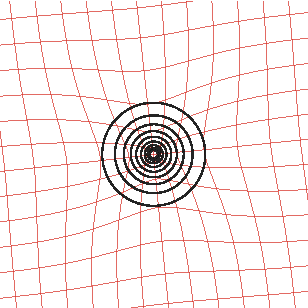
\includegraphics[width=.31\linewidth]{figures/monge-jacobian-pushforward-density/one-bump.pdf} &
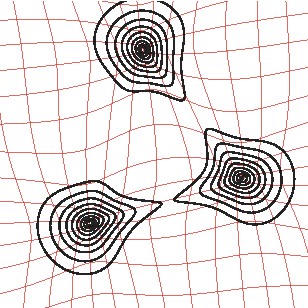
\includegraphics[width=.31\linewidth]{figures/monge-jacobian-pushforward-density/three-bumps.pdf} &
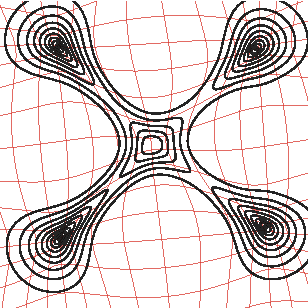
\includegraphics[width=.31\linewidth]{figures/monge-jacobian-pushforward-density/five-bumps.pdf} \\[-.1em]
\small one compression bump &
\small three compression bumps &
\small five compression bumps
\end{tabular}
	\caption{\emph{Jacobian determinant in the density push-forward formula.} The three panels show smooth diffeomorphisms that strongly compress a uniform source grid around one, three, and five centers. The deformed grid is drawn as a dense red mesh, and the pushed density is shown through black level sets of $\density{\be}(y)=|\det \T'(\T^{-1}y)|^{-1}$. The tighter crop focuses on the bump region, where small grid cells coincide with large values of the pushed density.}
\label{fig:monge-jacobian-pushforward-density}
\end{figure}


\begin{rem}[Probabilistic interpretation]
\index{probabilistic coupling}% strictindex
Let $X:\Omega\to\X$ be a random variable defined on an abstract probability
space $(\Omega,\Ff,\PP)$. Its law, or probability distribution, is the
push-forward of $\PP$ by $X$, namely $\al=X_\sharp\PP$.
\index{random variable}% strictindex
\index{push-forward}% strictindex
%
Applying another push-forward $\be = \T_\sharp\al$ for $\T : \X \rightarrow \Y$, following~\eqref{eq-push-fwd}, is equivalent to defining another random variable $Y=\T(X)$, namely $\omega \in \Om \mapsto \T(X(\omega)) \in \Y$. Indeed
\[
	\be=\T_\sharp\al=\T_\sharp(X_\sharp\PP)=(\T\circ X)_\sharp\PP,
\]
so $\be$ is the law of $Y$.
%
Thus, if $x$ is sampled according to the law $\al$, then $y=\T(x)$ is sampled according to the law $\be$.
\end{rem}

%%%%%%%%%%%%%%%%%%%%%%%%%%%%%%%%%%%%%%%%%%%%%%%%%%%%%%%%%%%%%%%%%%%%%%%%%%%
\section{Monge's Formulation}
\index{Monge!problem}% strictindex
\label{sec-monge-formulation}
\label{sec-continuous-monge}

Monge's problem asks for a deterministic map transporting one law onto another while minimizing a prescribed cost. This is the original formulation introduced by Monge in his memoir on the ``d\'eblai et remblai'' problem~\cite{Monge1781}. It is geometrically direct, because every source point is assigned one destination, but it is also analytically fragile: the feasible set is non-convex, it can be empty, and a map cannot split mass. These limitations are precisely what motivate Kantorovich's relaxation in the next chapter.
\index{Kantorovich!relaxation}% strictindex

\paragraph{Monge problem.}

The deterministic transport constraint leads to the following optimization problem.
\index{Monge!problem}% strictindex
\begin{defn}[Monge problem and Monge map]\label{def-monge-problem}
	For $\al\in\Mm_+^1(\Xx)$, $\be\in\Mm_+^1(\Yy)$ and measurable $c:\Xx\times\Yy\to[0,+\infty]$, define
\eql{\label{eq-monge-continuous}
	\Monge_c(\al,\be)
	\eqdef
	\inf_{\T:\Xx\to\Yy\,\text{ measurable}}
	\enscond{\int_\Xx c(x,\T(x))\d\al(x)}{\T_\sharp\al=\be}.
}
	A feasible $\T$ is a Monge map; a minimizer is an optimal Monge map. The value is $+\infty$ if no feasible map exists.
\end{defn}
The constraint $\T_\sharp\al=\be$ means that $\T$ pushes the mass of $\al$ onto $\be$ in the sense of Definition~\ref{defn-pushfwd}.

A diffuse one-dimensional example makes the deterministic constraint visible without reducing the measures to point clouds. For the quadratic cost, the optimal map between an atomless source and an arbitrary target is the monotone rearrangement
\[
	\T=\cumul{\be}^{-1}\circ\cumul{\al},
\]
as proved in Theorem~\ref{prop-1d-quantile-map}. Figure~\ref{fig:monge-1d-map-mixtures} applies this formula to a two-component Gaussian mixture and a three-component Gaussian mixture. The left panel follows equal quantile levels from source to target; the right panel displays the resulting map directly.

\begin{figure}[H]
\centering
\begin{tabular}{@{}cc@{}}
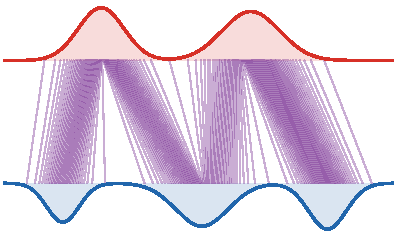
\includegraphics[width=.47\linewidth]{figures/monge-1d-map-mixtures/quantile-rays.pdf} &
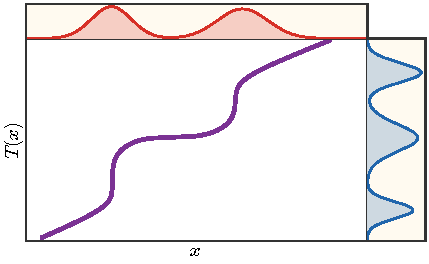
\includegraphics[width=.47\linewidth]{figures/monge-1d-map-mixtures/map-graph.pdf} \\[-.1em]
\small equal-quantile transport &
\small Monge map $y=\T(x)$
\end{tabular}
\caption{\emph{A one-dimensional Monge map between Gaussian mixtures.} The red source is a two-component mixture and the blue target is a three-component mixture. The left panel draws a dense family of equal-quantile transport rays without empirical atoms. The right panel shows the same monotone rearrangement as the graph of $\T=\cumul{\be}^{-1}\circ\cumul{\al}$, framed by the source and target densities. Its changes of slope encode the density balance $\density{\al}(x)=\T'(x)\density{\be}(\T(x))$ from Proposition~\ref{prop-push-forward-densities}.}
\label{fig:monge-1d-map-mixtures}
\index{Monge!map}% strictindex
\index{quantile!map}% strictindex
\end{figure}

\begin{prop}[Empirical Monge maps and matchings]\label{prop-empirical-monge-matching}
\index{Monge!problem}% strictindex
\index{empirical!Monge map}% strictindex
	Assume that the source atoms $x_1,\ldots,x_n$ are distinct and that
	\[
		\al=\frac1n\sum_{i=1}^n\de_{x_i},
		\qquad
		\be=\frac1n\sum_{j=1}^n\de_{y_j}.
	\]
	If $\T_\sharp\al=\be$, then for each distinct target value $z$ in the support of $\be$, exactly $n\be(\{z\})$ source atoms are mapped to $z$. In particular, if the $y_j$ are distinct, then there exists a permutation $\sigma\in\Perm(n)$ such that $\T(x_i)=y_{\sigma(i)}$ for all $i$. Conversely, every such assignment of source atoms to target atoms with the correct masses defines a feasible Monge map on the support of $\al$, and in the distinct-target case
\index{Monge!map}% strictindex
	\[
		\int_\Xx c(x,\T(x))\d\al(x)=\frac1n\sum_{i=1}^n c(x_i,y_{\sigma(i)}).
	\]
	The values of a feasible map away from $\{x_1,\ldots,x_n\}$ may be chosen arbitrarily, provided the resulting extension is measurable. If source locations are repeated, they should first be merged into atoms with larger masses; such atoms cannot be split by a Monge map.
\end{prop}
\begin{proof}
	Since $\T_\sharp\al=\be$, all images $\T(x_i)$ must belong to the support of $\be$; otherwise the push-forward would give positive mass to a point outside that support. For any target atom $z$,
\index{push-forward}% strictindex
	\[
		\be(\{z\})=\al(\T^{-1}(\{z\}))=\frac1n\#\enscond{i}{\T(x_i)=z}.
	\]
	This proves the counting statement. If all target atoms have mass $1/n$, each target receives exactly one source atom, which is a permutation. The converse and the cost identity follow by direct substitution.
\end{proof}

\begin{prop}[Existence of transport maps from atomless sources]\label{prop-existence-transport-map-atomless}
\index{transport!map}% strictindex
\index{measure!atomless}% strictindex
	Let $\al$ and $\be$ be Borel probability measures on Polish spaces, and assume that $\al$ is atomless. Then there exists a measurable map $\T$ such that $\T_\sharp\al=\be$.
\index{probability measure}% strictindex
\index{Polish space}% strictindex
\index{measure!atomless}% strictindex
\end{prop}
\begin{proof}
	A standard measure-isomorphism theorem identifies the atomless standard probability space $(\Xx,\al)$ with $([0,1],\mathrm{Leb})$, modulo null sets~\cite{bogachev2007measure}. It is therefore enough to construct a map from $[0,1]$ to the target law $\be$. Since the target is Polish, it is a standard Borel space; choose a Borel isomorphism $i$ from a full-$\be$ Borel subset of $\Yy$ onto a Borel subset of $[0,1]$. The generalized quantile of $i_\sharp\be$ pushes Lebesgue measure to $i_\sharp\be$. Composing it with $i^{-1}$ and with the source isomorphism gives the desired measurable map, after arbitrary definitions on the discarded null sets.
\index{Lebesgue measure}% strictindex
\index{transport!map}% strictindex
\index{generalized!inverse}% strictindex
\index{measure!isomorphism}% strictindex
\end{proof}

\begin{rem}[Feasibility versus optimality]
	An optimal map solving~\eqref{eq-monge-continuous} might fail to exist for two distinct reasons. First, the constraint set can be empty, for instance if $\al=\de_x$ and $\be$ is not a single Dirac mass. Proposition~\ref{prop-existence-transport-map-atomless} shows that non-atomicity of the source removes this feasibility obstruction. Second, even when feasible maps exist, the infimum may fail to be attained because the class of maps is not closed under weak limits.
\index{weak!limit}% strictindex
\index{Dirac mass}% strictindex
\end{rem}

\begin{example}[A splitting obstruction]\label{ex-splitting-obstruction}
\index{splitting obstruction}% strictindex
	Let $\al$ be uniform on $\{0\}\times[0,1]$ and let $\be$ be the average of the uniform laws on $\{-1\}\times[0,1]$ and $\{1\}\times[0,1]$. For the squared Euclidean cost, the relaxed plan that sends $(0,t)$ equally to $(-1,t)$ and $(1,t)$ has cost $1$, which is the smallest possible value because every target point is at horizontal distance $1$ from the source segment.

	No deterministic map can attain this value. Indeed, equality would force the vertical coordinate to remain equal to $t$ almost everywhere. If $A\subset[0,1]$ were the set of levels sent to the right segment, the target marginal would then require
	$|A\cap B|=|B|/2$ for every Borel set $B\subset[0,1]$, which is impossible by taking $B=A$. Feasible maps nevertheless approach cost $1$: partition $[0,1]$ into $n$ equal cells, send the lower half of each cell affinely onto the corresponding full cell on the left segment, and send the upper half similarly to the right segment. The vertical displacement is at most $1/(2n)$, so the costs converge to $1$. Thus the Monge infimum equals the relaxed value but is not attained~\cite{SantambrogioBook}.
\index{quadratic!cost}% strictindex
\index{Monge!problem}% strictindex
\end{example}

\begin{example}[Semi-discrete Monge maps]
\index{semi-discrete!Monge map}% strictindex
	The Monge formulation is not symmetric in $\al$ and $\be$. It makes sense, for instance, when $\al$ has a density with respect to Lebesgue measure and $\be$ is discrete. On $\Xx=\Yy=\RR^d$, let $\be=\sum_j b_j\delta_{y_j}$ be supported on $\{y_1,\ldots,y_m\}$. A map $\T$ such that $\T_\sharp\al=\be$ defines a segmentation of the space into cells
\index{Lebesgue measure}% strictindex
	$C_j\eqdef\T^{-1}(y_j)$ satisfying $\al(C_j)=b_j$.
	This is the semi-discrete setting. Chapter~\ref{sec-semidiscr-w1} explains how the cells become Laguerre cells for prescribed masses and ordinary Voronoi cells when the masses are free. Figure~\ref{fig:monge-semidiscrete-maps} shows two such equal-mass piecewise-constant maps: the color of each target atom matches the Laguerre cell that is sent to it. If one exchanges the roles of $\al$ and $\be$ so that $\al$ is discrete, then no valid $\T$ exists in general: it is not possible to push forward a discrete measure to a measure with density.
\index{Laguerre cell}% strictindex
\index{semi-discrete!OT}% strictindex
\index{push-forward}% strictindex
\index{Voronoi cell}% strictindex
\end{example}

\begin{figure}[ht]
\centering
\begin{tabular}{@{}cc@{}}
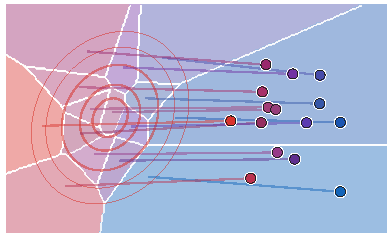
\includegraphics[width=.48\linewidth]{figures/monge-semidiscrete-maps/gaussian-to-discrete.pdf} &
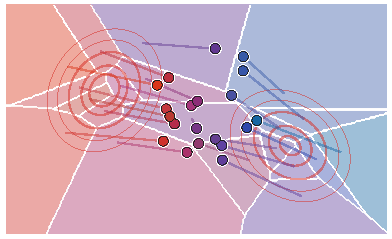
\includegraphics[width=.48\linewidth]{figures/monge-semidiscrete-maps/mixture-to-discrete.pdf} \\[-.1em]
\small Gaussian source to 15 atoms &
\index{Gaussian!measure}% strictindex
\small two-mode source to 20 atoms
\end{tabular}
\caption{\emph{Semi-discrete Monge maps.} The red contours show the continuous source density $\al$. The colored regions extend the numerical Laguerre cells over the whole displayed domain, while their masses are computed with respect to $\al$. The circular atoms form the discrete target $\be$. Their colors are tied to horizontal position, with a small random perturbation, and are reused for the cells. Faint segments connect cell barycenters to their images under the piecewise-constant Monge map.}
\label{fig:monge-semidiscrete-maps}
\index{semi-discrete!Monge map}% strictindex
\index{Laguerre cell}% strictindex
\end{figure}

Figure~\ref{fig:monge-color-transfer-rgb} shows a finite-dimensional instance of this deterministic viewpoint. The source and target measures are empirical color clouds in RGB space, and the map transports colors while leaving pixel positions fixed. Grayscale equalization is one-dimensional, but transferring a full color palette requires comparing empirical measures in a three-dimensional color space, for instance RGB or Lab. Early color-transfer methods used affine statistics or iterated one-dimensional projections~\cite{reinhard2001color,pitie2005n}; the latter viewpoint also underlies sliced-Wasserstein methods for texture mixing~\cite{rabin-ssvm-11}. The experiment below instead computes a genuine three-dimensional optimal assignment between two sampled RGB palettes.
\index{empirical!measure}% strictindex
\index{one-dimensional!projection}% strictindex

\begin{figure}[H]
\centering
\begin{tabular}{@{}ccccc@{}}
\small source & \small $t=1/3$ & \small $t=2/3$ & \small transported & \small target \\[-.15em]
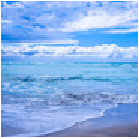
\includegraphics[width=.17\linewidth]{figures/monge-color-transfer-rgb/image-t000.pdf} &
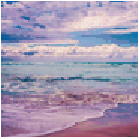
\includegraphics[width=.17\linewidth]{figures/monge-color-transfer-rgb/image-t033.pdf} &
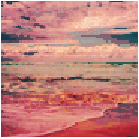
\includegraphics[width=.17\linewidth]{figures/monge-color-transfer-rgb/image-t067.pdf} &
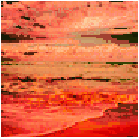
\includegraphics[width=.17\linewidth]{figures/monge-color-transfer-rgb/image-t100.pdf} &
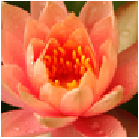
\includegraphics[width=.17\linewidth]{figures/monge-color-transfer-rgb/image-target.pdf} \\[-.1em]
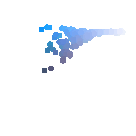
\includegraphics[width=.17\linewidth]{figures/monge-color-transfer-rgb/rgb-t000.pdf} &
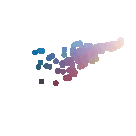
\includegraphics[width=.17\linewidth]{figures/monge-color-transfer-rgb/rgb-t033.pdf} &
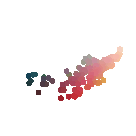
\includegraphics[width=.17\linewidth]{figures/monge-color-transfer-rgb/rgb-t067.pdf} &
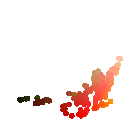
\includegraphics[width=.17\linewidth]{figures/monge-color-transfer-rgb/rgb-t100.pdf} &
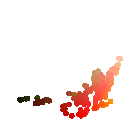
\includegraphics[width=.17\linewidth]{figures/monge-color-transfer-rgb/rgb-target.pdf}
\end{tabular}
\caption{\emph{Color transfer as a Monge map in RGB space, from a beach photograph to a flower photograph.} The top row applies the palette map to the source image; the bottom row shows the empirical color clouds in the RGB cube. Only colors are transported here, not pixel locations.}
\label{fig:monge-color-transfer-rgb}
\end{figure}

\paragraph{Monge distance.}
\index{Monge!distance}% strictindex

Specializing the cost to a power of a metric produces a directed transport distance.
\begin{defn}[Directed Monge distance]\label{def-directed-monge-distance}
Let $(\Xx,d)$ be a metric space and $1\leq p<+\infty$. For probability measures with finite $p$th moments, define
\eql{\label{eq-monge-distance}
\index{Monge!distance}% strictindex
	\tilde\Wass_p(\al,\be)^p
	\eqdef
	\inf_{\T:\Xx\to\Xx\,\text{ measurable}}
	\enscond{\int_\Xx d(x,\T(x))^p\d\al(x)}{\T_\sharp\al=\be}.
}
The value is $+\infty$ when the constraint set is empty.
\end{defn}

\begin{example}[Book-shifting in the Monge problem]\label{ex-monge-book-shifting-w1}
\index{book-shifting}% strictindex
\index{Wasserstein!W1 non-uniqueness@$\Wass_1$ non-uniqueness}% strictindex
	This is the continuous counterpart of the discrete book-shifting construction in Example~\ref{ex-book-shifting-w1}; it exhibits the same non-uniqueness mechanism for the linear cost.
	Let $\al=\frac12\mathds{1}_{[0,2]}(x)\d x$ and
	$\be=\frac12\mathds{1}_{[1,3]}(y)\d y$.
	The monotone translation $T_{\rm tr}(x)=x+1$ pushes $\al$ to $\be$. For the cost $|x-y|$, it is not the only optimal Monge map. The book-shifting map
\index{book-shifting}% strictindex
	$T_{\rm book}(x)=x+2$ for $0\leq x\leq1$ and
	$T_{\rm book}(x)=x$ for $1<x\leq2$ also satisfies
	$(T_{\rm book})_\sharp\al=\be$: it keeps the overlapping interval $[1,2]$ fixed and sends the left interval $[0,1]$ to the uncovered interval $[2,3]$. For any admissible map $T_\sharp\al=\be$,
	\[
		\int |T(x)-x|\d\al(x)
		\geq
		\int (T(x)-x)\d\al(x)
		=
		\int y\d\be(y)-\int x\d\al(x)
		=1.
	\]
	Both $T_{\rm tr}$ and $T_{\rm book}$ satisfy $T(x)\geq x$ for $\al$-almost every $x$, hence both saturate this lower bound and are optimal for the Monge value $\tilde\Wass_1$. More generally, one may replace the map $x\mapsto x+2$ on $[0,1]$ by any measure-preserving map from $[0,1]$ to $[2,3]$, while keeping the identity on $[1,2]$. The flatness is specific to the linear cost: for $p>1$, strict convexity selects the monotone translation.
\index{measure-preserving!map}% strictindex
\index{Monge!map}% strictindex
\end{example}

\begin{prop}[Directed Monge distance]\label{prop-directed-monge-distance}
\index{Monge!distance}% strictindex
	Let $\Xx=\Yy$ be a Polish metric space and $1\leq p<+\infty$. On probability measures with finite $p$-th moment, the quantity $\tilde\Wass_p$ is nonnegative, vanishes only on the diagonal, and satisfies the triangle inequality. It is therefore a directed extended distance: it need not be symmetric and may take the value $+\infty$.
\index{triangle inequality}% strictindex
\end{prop}
\begin{proof}
	Nonnegativity is immediate. If $\tilde\Wass_p(\al,\be)=0$, choose feasible maps $\T_k$ with $\int d(x,\T_k(x))^p\d\al(x)\to0$. For every bounded $1$-Lipschitz function $h$,
\index{Lipschitz!function}% strictindex
	\[
		\left|\int h\d\be-\int h\d\al\right|
		=
		\left|\int h(\T_k(x))-h(x)\d\al(x)\right|
		\leq
		\left(\int d(x,\T_k(x))^p\d\al(x)\right)^{1/p}
		\longrightarrow0.
	\]
	Since bounded Lipschitz functions separate probability measures on Polish metric spaces, $\al=\be$. Conversely, the identity map shows that $\tilde\Wass_p(\al,\al)=0$.
\index{probability measure}% strictindex
\index{Lipschitz!function}% strictindex

	We prove the triangle inequality. If either $\tilde\Wass_p(\al,\ga)$ or $\tilde\Wass_p(\ga,\be)$ is infinite, the claim is automatic. If both are finite, feasible maps $S_\sharp\al=\ga$ and $T_\sharp\ga=\be$ exist, so their composition is feasible from $\al$ to $\be$; in particular, the left-hand side is finite. Fix $\epsilon>0$ and choose $\epsilon$-minimizers satisfying
\index{triangle inequality}% strictindex
	\[
		\Ee_\al(S)^{1/p}\leq\tilde\Wass_p(\al,\ga)+\epsilon,
		\qquad
		\Ee_\ga(T)^{1/p}\leq\tilde\Wass_p(\ga,\be)+\epsilon.
	\]
	The composed map is feasible from $\al$ to $\be$, and Minkowski's inequality gives
\index{Minkowski inequality}% strictindex
	\[
	\begin{aligned}
		\tilde\Wass_p(\al,\be)
		&\leq
		\left(\int d(x,T(S(x)))^p\d\al(x)\right)^{1/p} \\
		&\leq
		\left(\int d(x,S(x))^p\d\al(x)\right)^{1/p}
		+
		\left(\int d(S(x),T(S(x)))^p\d\al(x)\right)^{1/p} \\
		&=
		\Ee_\al(S)^{1/p}+\Ee_\ga(T)^{1/p}
		\leq
		\tilde\Wass_p(\al,\ga)+\tilde\Wass_p(\ga,\be)+2\epsilon.
	\end{aligned}
	\]
	Letting $\epsilon\to0$ gives the result.
\end{proof}

The directed value $\tilde\Wass_p$ is useful conceptually, but it is too rigid to be the main distance between measures: it can be infinite and asymmetric. The Kantorovich formulation remedies both issues by replacing maps with couplings.

%%%%%%%%%%%%%%%%%%%%%%%%%%%%%%%%%%%%%%%%%%%%%%%%%%%%%%%%%%%%%%%%%%%%%%%%%%%
\section{Existence and Uniqueness of the Monge Map}
\index{Monge!problem}% strictindex
\label{sec-monge-existence-uniqueness}

This section records the main regimes where Monge's deterministic formulation becomes well posed. Brenier's theorem is the central result: for the squared Euclidean cost, absolute continuity of the source restores existence, uniqueness and convex-potential structure.
\index{Brenier!theorem}% strictindex
\index{absolute continuity}% strictindex
\index{convex!potential}% strictindex

\paragraph{Brenier's theorem.}

Brenier's theorem~\cite{MR923203,Brenier91} ensures that, in $\RR^d$ for the quadratic cost, absolute continuity of the source is enough for Monge's problem to have a unique solution. It also gives the decisive structural description of this solution: the optimal map is not an arbitrary map, but the gradient of a convex potential.
\index{quadratic!cost}% strictindex
\index{Monge!problem}% strictindex

\begin{thm}[Brenier]\label{thm-brenier}
	Let $\al,\be\in\Mm_+^1(\RR^d)$ have finite second moments, and assume that $\al$ is absolutely continuous with respect to Lebesgue measure. For the quadratic cost $c(x,y)=\norm{x-y}^2$, there exists a convex function $\phi:\RR^d\to\RR\cup\{+\infty\}$ such that
\index{Lebesgue measure}% strictindex
\index{convex!function}% strictindex
	\[
		\T=\nabla\phi,
		\qquad
		\T_\sharp\al=\be,
	\]
	and $\T$ is the unique optimal Monge map $\al$-almost everywhere. The optimal Kantorovich plan is $(\Id,\T)_\sharp\al$.
\index{Monge!problem}% strictindex
\end{thm}
\begin{proof}
	The proof uses the Kantorovich relaxation and duality developed later in Chapter~\ref{sec-dual}. Apply Proposition~\ref{prop-quadratic-dual-attainment} to the normalized cost and multiply its dual potentials by two. This supplies optimal extended $c$-concave potentials $(f,g)$ for the cost $\norm{x-y}^2$, finite almost everywhere and integrable against their respective marginals. Define
	\[
		\phi(x)\eqdef\frac12\norm{x}^2-\frac12 f(x),
		\qquad
		\psi(y)\eqdef\frac12\norm{y}^2-\frac12 g(y).
	\]
	The $c$-concavity of $f$ makes $\phi$ convex. Dual feasibility is equivalent to $\phi(x)+\psi(y)\geq\dotp{x}{y}$, and equality holds for almost every pair under any optimal plan. Replacing $\psi$ by the convex conjugate $\phi^*$ therefore yields the Fenchel equality $\phi(x)+\phi^*(y)=\dotp{x}{y}$ on the optimal relation, hence $y\in\partial\phi(x)$. Since $\al$ has a density and convex functions are differentiable Lebesgue-almost everywhere, $\partial\phi(x)=\{\nabla\phi(x)\}$ for $\al$-almost every $x$. Every optimal plan is therefore concentrated on the same graph, which proves existence and uniqueness of both the optimal plan and the Monge map. Related results for more general strictly convex costs are developed in~\cite{gangbo1996geometry,caffarelli2002constructing,Villani09}.
\index{subdifferential}% strictindex
\index{optimal coupling}% strictindex
\index{Kantorovich!relaxation}% strictindex
\index{Kantorovich!duality}% strictindex
\index{quadratic!cost}% strictindex
\index{Brenier!theorem}% strictindex
\end{proof}

Brenier's theorem is the higher-dimensional analogue of the one-dimensional monotone rearrangement theorem. In one dimension, the derivative of a convex function is an increasing map; in several dimensions, the corresponding object is the gradient of a convex function. Such gradients are monotone fields:
\index{convex!function}% strictindex
\index{monotone!rearrangement}% strictindex
\[
	\dotp{\nabla\phi(x)-\nabla\phi(x')}{x-x'}\geq0.
\]

\begin{rem}[Monotone fields need not be gradients]
\index{monotone!field}% strictindex
\index{gradient!field}% strictindex
	In dimensions larger than one, not all monotone fields are gradients of convex functions. Consider in $\RR^2$ the rotation matrix
\index{convex!function}% strictindex
	$R_\theta=\begin{psmallmatrix}
	\cos\theta & -\sin\theta\\
	\sin\theta & \cos\theta
	\end{psmallmatrix}$.
	The linear map $x\mapsto R_\theta x$ is monotone as soon as $|\theta|\leq\pi/2$, because
	\[
		\dotp{R_\theta x-R_\theta x'}{x-x'}
		=
		\dotp{R_\theta(x-x')}{x-x'}
		=
		\cos(\theta)\norm{x-x'}^2\geq0.
	\]
	However, for $\theta\neq0$, $R_\theta$ is not symmetric and therefore cannot be the gradient of a scalar potential. Indeed, if a linear field $Ax$ equals $\nabla\phi(x)$, then its Jacobian $A$ must be symmetric; equivalently, a quadratic potential $\phi(x)=\dotp{Bx}{x}/2$ has gradient $((B+B^\top)/2)x$. Thus monotonicity is weaker than Brenier optimality in dimension $d\geq2$.
\index{quadratic!potential}% strictindex
\end{rem}

\begin{defn}[Measures not charging hypersurfaces]\label{defn-not-charging-hypersurfaces}
\index{hypersurface}% strictindex
	A Borel measure $\al$ on $\RR^d$ does not charge hypersurfaces if $\al(S)=0$ for every countably $(d-1)$-rectifiable set $S$, i.e.\ every set that can be covered, up to an $\mathcal H^{d-1}$-null set, by countably many $C^1$ hypersurfaces.
\index{rectifiable set}% strictindex
\index{Hausdorff measure}% strictindex
\index{Borel measure}% strictindex
\end{defn}

\begin{rem}[A sharp source hypothesis]
\index{Brenier!source hypothesis}% strictindex
	The absolute-continuity assumption in Brenier's theorem can be weakened: for the quadratic cost, it is enough that $\al$ does not charge hypersurfaces~\cite{gangbo1996geometry,Villani09,SantambrogioBook}. The reason is that the set where a convex potential has a genuinely multi-valued subdifferential is contained in a countable union of lower-dimensional pieces. This condition is close to sharp. If the source gives positive mass to a segment or a hypersurface, the subdifferential may be multi-valued on a set of positive $\al$-mass, and the optimal relaxed plan may need to split mass, as in Example~\ref{ex-splitting-obstruction}.
\index{multi-valued subdifferential}% strictindex
\index{lower-dimensional set}% strictindex
\index{hypersurface}% strictindex
\index{subdifferential}% strictindex
\index{Brenier!theorem}% strictindex
\index{splitting obstruction}% strictindex
\index{absolute continuity}% strictindex
\index{convex!potential}% strictindex
\index{quadratic!cost}% strictindex
\end{rem}

\paragraph{Radial measures.}
\index{radial measure}% strictindex

Radial symmetry gives a useful higher-dimensional case where the Brenier map reduces to a one-dimensional monotone rearrangement. A measure $\al$ on $\RR^d$ is radial if $Q_\sharp\al=\al$ for every orthogonal map $Q$. Such a measure is determined by the law of the radius $\norm{x}$, and the optimal map transports this radius while keeping the angular direction fixed.
\index{Brenier!map}% strictindex
\index{monotone!rearrangement}% strictindex

\begin{prop}[Optimal transport between radial measures]\label{prop-radial-transport}
	Let $\al,\be\in\Mm_+^1(\RR^d)$ be radial probability measures with finite second moments, and assume that $\al$ is absolutely continuous with respect to Lebesgue measure. Define their radial distribution functions
	\[
		F_\al(r)\eqdef \al(\{x:\norm{x}\leq r\}),
		\qquad
		F_\be(r)\eqdef \be(\{y:\norm{y}\leq r\}),
		\qquad r\geq0,
	\]
	and let $F_\be^{-1}(u)\eqdef\inf\{r\geq0:F_\be(r)\geq u\}$ be the generalized inverse.
	Set $\tau(r)\eqdef F_\be^{-1}(F_\al(r))$.
	Then the quadratic Brenier map from $\al$ to $\be$ is the radial map
	\[
		\T(0)=0,
		\qquad
		\T(x)=\frac{\tau(\norm{x})}{\norm{x}}x
		\quad\text{for }x\neq0.
	\]
	Moreover, if $\al_R=(x\mapsto\norm{x})_\sharp\al$ is the law of the source radius, then
	\[
		\Wass_2^2(\al,\be)
		=
		\int_0^\infty |r-\tau(r)|^2\,\d\al_R(r).
	\]
\end{prop}
\begin{proof}
	Let $\al_R=(\norm{\cdot})_\sharp\al$ and $\be_R=(\norm{\cdot})_\sharp\be$ be the radial laws. Since $\al$ is absolutely continuous, $\al_R$ has no atoms. The map $\tau=F_\be^{-1}\circ F_\al$ is therefore the monotone one-dimensional transport from $\al_R$ to $\be_R$. If $X\sim\al$ and $R=\norm{X}$, then $\tau(R)$ has law $\be_R$. Moreover, by radiality, the conditional direction $X/\norm{X}$ given $R=r$ is uniform on the sphere for $\al_R$-a.e.\ $r>0$. Thus $\T$ changes only the radius, from $R$ to $\tau(R)$, and keeps the uniform angular distribution. It follows that $\T_\sharp\al$ is radial with radial law $\be_R$, hence $\T_\sharp\al=\be$.

	It remains to check optimality. The function $\tau$ is nondecreasing and nonnegative. Define $\psi(r)\eqdef\int_0^r\tau(s)\d s$ on $\RR_+$. Then $\psi$ is convex and nondecreasing, so $\phi(x)\eqdef\psi(\norm{x})$ is convex on $\RR^d$. Since $\al$ is absolutely continuous, it does not charge the origin nor the radii where the monotone function $\tau$ is discontinuous. Thus
	$\nabla\phi(x)=\tau(\norm{x})x/\norm{x}=\T(x)$ for $\al$-a.e.\ $x$.
	The map $\T$ is therefore a gradient of a convex potential and pushes $\al$ to $\be$. Brenier's theorem identifies it as the unique quadratic optimal Monge map. The displayed cost formula follows by substituting $\T(x)$ in $\int\norm{x-\T(x)}^2\d\al(x)$.
\index{convex!potential}% strictindex
\index{one-dimensional!transport}% strictindex
\end{proof}

If $\al$ is not absolutely continuous, the same radial idea is still useful but has to be interpreted at the level of couplings of the radial variables: atoms on spheres may have to be split, so a Monge map need not exist.
\index{radial coupling}% strictindex

\paragraph{Polar factorization.}
\index{polar factorization}% strictindex

Brenier's theorem does more than solve one transport problem: it provides a canonical way to extract the ``monotone part'' of a nondegenerate map. Suppose one starts from a square-integrable deformation $u:\Omega\to\RR^d$, for instance a velocity snapshot, an image deformation or a generative map. The law $\be=u_\sharp\lambda$ records where the mass ends up, but it forgets how the points of $\Omega$ were labelled before being sent there. Brenier's polar factorization~\cite{MR923203,Brenier91} separates these two effects. A measure-preserving rearrangement $s$ first changes the labels without changing the source law; the unique convex-gradient map $\nabla\phi$ then sends the uniform source to the output law. Thus the Brenier factor is the canonical optimal-transport representative among all maps with the same image distribution.
\index{measure-preserving!map}% strictindex
\index{Brenier!theorem}% strictindex
\index{Brenier!factor}% strictindex

\begin{prop}[Polar factorization]\label{prop-polar-factorization}
	Let $\Omega\subset\RR^d$ be a bounded domain endowed with normalized Lebesgue measure $\lambda$, and let $u\in L^2(\Omega;\RR^d)$. Assume that the image law $\be=u_\sharp\lambda$ is absolutely continuous with respect to Lebesgue measure. Then there exist a measure-preserving map $s:\Omega\to\Omega$ and a convex function $\phi$ such that
\index{Lebesgue measure}% strictindex
\index{convex!function}% strictindex
	\[
		u=\nabla\phi\circ s
		\qquad \lambda\text{-a.e.}
	\]
	The Brenier factor $\nabla\phi$ and the rearrangement $s$ are unique $\lambda$-almost everywhere.
\index{Brenier!factor}% strictindex
\end{prop}
\begin{proof}
	By Brenier's theorem there is a unique convex-gradient map $\T=\nabla\phi$ transporting $\lambda$ to $\be$. Since $\be$ is also absolutely continuous, the reverse Brenier map $S$ transporting $\be$ to $\lambda$ exists, and the two maps are inverse almost everywhere: $\T\circ S=\Id$ $\be$-almost everywhere and $S\circ\T=\Id$ $\lambda$-almost everywhere. Set $s\eqdef S\circ u$. Then
	\[
		s_\sharp\lambda=S_\sharp(u_\sharp\lambda)=S_\sharp\be=\lambda,
		\qquad
		\T\circ s=\T\circ S\circ u=u
		\quad\lambda\text{-a.e.}
	\]
	Thus $s$ is measure preserving and gives the announced factorization. Uniqueness of $\T$ follows from Brenier's theorem, and then $s=S\circ u$ is unique almost everywhere.
\index{measure-preserving!map}% strictindex
\index{Brenier!theorem}% strictindex
\end{proof}

The absolute-continuity assumption is a transparent sufficient form of Brenier's nondegeneracy hypothesis: $u^{-1}(N)$ must be $\lambda$-null whenever $N\subset\RR^d$ is Lebesgue-null. Without such a hypothesis, a deterministic factorization can fail or the rearrangement can be nonunique; the always-available relaxation replaces $s$ by a measure-preserving plan.

Figure~\ref{fig:monge-polar-factorization} separates these two factors on a colored grid. Its three panels display the initial coordinates $x$, the relabeled coordinates $s(x)$, and the factorized deformation $u(x)=(\nabla\phi\circ s)(x)$. The map $s$ swirls the grid inside the square while preserving area, whereas $\nabla\phi$ is a symmetric positive definite affine map and hence the gradient of a convex quadratic potential.
\index{measure-preserving!map}% strictindex
\index{convex!potential}% strictindex

\begin{figure}[htbp]
\centering
\begin{tabular}{@{}ccc@{}}

\includegraphics[width=.30\linewidth]{figures/monge-polar-factorization/source-grid.pdf} &
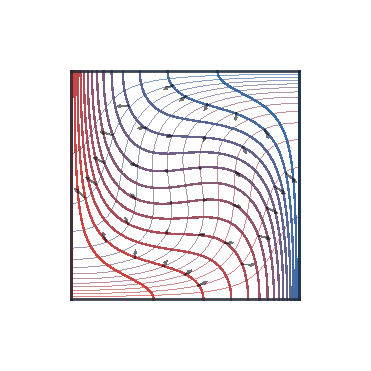
\includegraphics[width=.30\linewidth]{figures/monge-polar-factorization/relabeling-grid.pdf} &
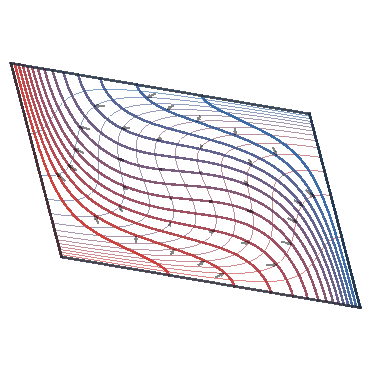
\includegraphics[width=.30\linewidth]{figures/monge-polar-factorization/final-grid.pdf} \\[-.1em]
\small $x$ & \small $s(x)$ & \small $u(x)=(\nabla\phi\circ s)(x)$
\end{tabular}
\caption{\emph{Polar factorization as a relabeling followed by a Brenier map.} From left to right, the panels show $x$, $s(x)$ with $s_\sharp\lambda=\lambda$, and $u(x)=\nabla\phi(s(x))$. Here $s$ is generated by the area-preserving flow of a divergence-free Hamiltonian vector field, while the Brenier factor is the symmetric positive definite affine map $\nabla\phi(z)=Bz$. Faint arrows indicate the successive maps.}
\index{polar factorization}% strictindex
\index{Brenier!map}% strictindex
\label{fig:monge-polar-factorization}
\end{figure}

The name is meant to echo the usual polar decomposition of matrices. This analogy becomes literal for linear maps under the Gaussian reference measure. If $X\sim\Gaussian(0,\Id)$ and $u(x)=Ax$, then $u_\sharp\Gaussian(0,\Id)=\Gaussian(0,AA^\top)$. The Brenier map from $\Gaussian(0,\Id)$ to this Gaussian is $x\mapsto Sx$, where $S=(AA^\top)^{1/2}$ is symmetric positive semidefinite. Hence the decomposition $u=\nabla\phi\circ s$ reads
\index{matrix!polar decomposition}% strictindex
\index{reference!measure}% strictindex
\index{Brenier!map}% strictindex
\index{Gaussian!measure}% strictindex
$A=SO$, where $O=S^{-1}A$ is orthogonal when $A$ is invertible. If $A$ is singular, $S^\dagger A$ is the canonical partial isometry on $(\ker A)^\perp$; because $A$ is square, it can be extended arbitrarily to an orthogonal matrix $O$ on all of $\RR^d$ while preserving $A=SO$. This orthogonal extension, rather than the unextended partial isometry, preserves the standard Gaussian law. The factor $Sx$ is the convex-gradient transport part, while $Ox$ is the measure-preserving relabeling.
\index{matrix!polar decomposition}% strictindex
\index{polar factorization}% strictindex

\paragraph{Displacement interpolation.}
\index{displacement interpolation}% strictindex
\label{sec-monge-interpolation}

An optimal map does not only match two endpoint measures; it also tells how to draw a path between them. The construction is Lagrangian and geometric: each particle keeps its identity and travels at constant speed from its initial position to its image under the transport map.
\index{transport!map}% strictindex

\begin{defn}[Monge and McCann displacement interpolation]\label{def-monge-mccann-interpolation}
\index{Monge!interpolation}% strictindex
	If $\T_\sharp\al=\be$, the Monge interpolation generated by $\T$ is the curve
	\[
		\T_t(x)\eqdef(1-t)x+t\T(x),
		\qquad
		\al_t\eqdef(\T_t)_\sharp\al,
		\qquad t\in[0,1].
	\]
	For the quadratic cost, when $\T$ is the optimal Brenier map, this curve is called McCann's displacement interpolation.
\index{displacement interpolation}% strictindex
\end{defn}
McCann's displacement convexity theory~\cite{mccann1997convexity} clarifies the geometric meaning of interpolating along Brenier maps; this is the language of Wasserstein geodesics used later for barycenters in Section~\ref{sec-barycenters} and for gradient flows in Chapter~\ref{sec-wasserstein-gradient-flows}. If no Monge map exists, or if the optimal object splits mass, the same straight-line idea is applied to each active pair of a coupling, as explained in the Kantorovich interpolation of Section~\ref{sec-kantorovich-plan-interpolation}. The following proposition makes the constant-speed property precise for the directed Monge value.
\index{Brenier!map}% strictindex
\index{Monge!problem}% strictindex
\index{Wasserstein!geodesic}% strictindex
\index{gradient!flow}% strictindex
\index{Wasserstein!gradient flow}% strictindex
\index{Kantorovich!interpolation}% strictindex
\index{displacement convexity}% strictindex
\index{Monge!interpolation}% strictindex
\index{quadratic!cost}% strictindex

\begin{prop}[Directed Monge displacement geodesics]\label{prop-monge-displacement-geodesic}
\index{Monge!geodesic}% strictindex
	Let $1\leq p<+\infty$, let $\al,\be\in\Mm_+^1(\RR^d)$ have finite $p$-th moments, and let $\T$ be an optimal map for $\tilde\Wass_p(\al,\be)$ in~\eqref{eq-monge-distance}. Set $\al_t=(\T_t)_\sharp\al$ with $\T_t=(1-t)\Id+t\T$. Assume that, for every $t<1$, $\T_t$ is one-to-one on a full $\al$-measure Borel set. Its inverse on the image of that set is then measurable and defined $\al_t$-almost everywhere. For $0\leq s\leq t\leq1$,
\index{Borel set}% strictindex
\index{Monge!distance}% strictindex
	\[
		\tilde\Wass_p(\al_s,\al_t)=(t-s)\tilde\Wass_p(\al,\be).
	\]
	Thus $t\mapsto\al_t$ is an oriented constant-speed geodesic for the directed Monge distance. In particular, for $p=2$, this applies to the Brenier map under the hypotheses of Theorem~\ref{thm-brenier}.
\index{constant-speed geodesic}% strictindex
\index{Brenier!map}% strictindex
\end{prop}
\begin{proof}
	The case $s=t$ is trivial, so assume $s<t$. Since $s<1$, the inverse $\T_s^{-1}$ is defined $\al_s$-almost everywhere along the transported particles. Define
	$S_{s,t}\eqdef\T_t\circ\T_s^{-1}$ $\al_s$-a.e.
	Then $(S_{s,t})_\sharp\al_s=\al_t$, and, using the optimality of $\T$,
	\[
		\tilde\Wass_p(\al_s,\al_t)^p
		\leq
		\int \norm{S_{s,t}(z)-z}^p\d\al_s(z)
		=
		\int \norm{\T_t(x)-\T_s(x)}^p\d\al(x)
		=
		(t-s)^p\tilde\Wass_p(\al,\be)^p.
	\]
	The same particle construction gives $\tilde\Wass_p(\al,\al_s)\leq s\tilde\Wass_p(\al,\be)$. If $t<1$, the map $\T\circ\T_t^{-1}$ sends $\al_t$ to $\be$ and gives $\tilde\Wass_p(\al_t,\be)\leq(1-t)\tilde\Wass_p(\al,\be)$; if $t=1$, this latter distance is zero. Using the triangle inequality from Proposition~\ref{prop-directed-monge-distance},
\index{triangle inequality}% strictindex
\index{Monge!distance}% strictindex
	\[
		\tilde\Wass_p(\al,\be)
		\leq
		\tilde\Wass_p(\al,\al_s)+\tilde\Wass_p(\al_s,\al_t)+\tilde\Wass_p(\al_t,\be)
		\leq
		s\tilde\Wass_p(\al,\be)+\tilde\Wass_p(\al_s,\al_t)+(1-t)\tilde\Wass_p(\al,\be).
	\]
	Hence $\tilde\Wass_p(\al_s,\al_t)\geq(t-s)\tilde\Wass_p(\al,\be)$, which proves equality. For a Brenier map $\T=\nabla\phi$, the map $\T_t$ is the gradient of
\index{Brenier!map}% strictindex
	\(x\mapsto (1-t)\frac{\norm{x}^2}{2}+t\phi(x)\),
	which is $(1-t)$-strongly convex for every $t<1$. On the full-measure set where $\phi$ is differentiable, this gives
	$\dotp{\T_t(x)-\T_t(y)}{x-y}\geq(1-t)\norm{x-y}^2$, so $\T_t$ is injective there. This gives the last claim.
\end{proof}

Figure~\ref{fig:monge-shape-mccann-interpolation} illustrates this displacement geodesic on two non-convex silhouettes, both through representative particle paths and through the evolving transported density.

\begin{figure}[htbp]
\centering
\begin{tabular}{@{}ccccc@{}}
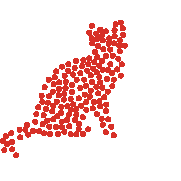
\includegraphics[width=.17\linewidth]{figures/monge-shape-mccann-interpolation/particles-t000.pdf} &
\index{McCann!interpolation}% strictindex
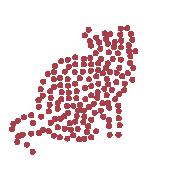
\includegraphics[width=.17\linewidth]{figures/monge-shape-mccann-interpolation/particles-t025.pdf} &
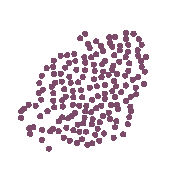
\includegraphics[width=.17\linewidth]{figures/monge-shape-mccann-interpolation/particles-t050.pdf} &
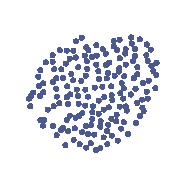
\includegraphics[width=.17\linewidth]{figures/monge-shape-mccann-interpolation/particles-t075.pdf} &
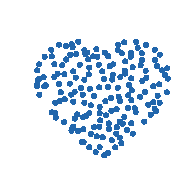
\includegraphics[width=.17\linewidth]{figures/monge-shape-mccann-interpolation/particles-t100.pdf} \\[-.1em]
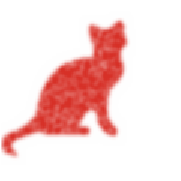
\includegraphics[width=.17\linewidth]{figures/monge-shape-mccann-interpolation/density-t000.pdf} &
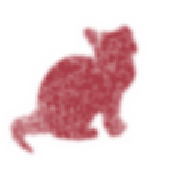
\includegraphics[width=.17\linewidth]{figures/monge-shape-mccann-interpolation/density-t025.pdf} &
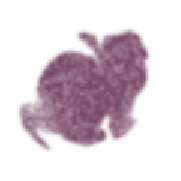
\includegraphics[width=.17\linewidth]{figures/monge-shape-mccann-interpolation/density-t050.pdf} &
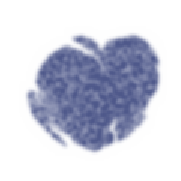
\includegraphics[width=.17\linewidth]{figures/monge-shape-mccann-interpolation/density-t075.pdf} &
\index{McCann!interpolation}% strictindex
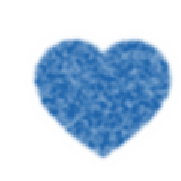
\includegraphics[width=.17\linewidth]{figures/monge-shape-mccann-interpolation/density-t100.pdf} \\[-.1em]
\small $t=0$ & \small $t=1/4$ & \small $t=1/2$ & \small $t=3/4$ & \small $t=1$
\end{tabular}
\caption{\emph{McCann displacement interpolation between a cat silhouette and a heart silhouette.} The first row displays a small farthest-point subset of transported particles along $T_t(x)=(1-t)x+tT(x)$. The second row renders kernel-smoothed densities from a denser transported cloud as color images: white means zero density, while high density saturates in the red-to-blue interpolation color of the corresponding time.}
\index{displacement interpolation}% strictindex
\label{fig:monge-shape-mccann-interpolation}
\end{figure}

Caffarelli's regularity theory, discussed next, explains when the convex potential is actually smooth enough to define a classical deformation.
\index{regularity theory}% strictindex
\index{Caffarelli regularity}% strictindex
\index{convex!potential}% strictindex

\paragraph{Regularity and the Monge--Amp\`ere equation.}
\index{Monge-Ampere@Monge--Amp\`ere!equation}% strictindex

The previous results identify the optimal map; regularity theory asks when this map is a classical smooth deformation rather than only an almost-everywhere gradient. For quadratic costs this question becomes the regularity theory of the Monge--Amp\`ere equation.
\index{quadratic!cost}% strictindex

\begin{prop}[Caffarelli regularity]\label{prop-caffarelli-regularity}
\index{Caffarelli regularity}% strictindex
	Let $\Omega,\Lambda\subset\RR^d$ be bounded uniformly convex domains with $C^2$ boundaries. Let $\al=\density{\al}(x)\d x$ and $\be=\density{\be}(y)\d y$ be supported on $\Omega$ and $\Lambda$, respectively, with
	\[
		0<m\leq\density{\al},\density{\be}\leq M<+\infty.
	\]
	If $\density{\al}\in C^\alpha(\overline\Omega)$ and $\density{\be}\in C^\alpha(\overline\Lambda)$ for some $\alpha\in(0,1)$, then the Brenier potential $\phi$ is strictly convex in $\Omega$ and belongs to $C^{2,\alpha}_{\mathrm{loc}}(\Omega)$. Consequently, $\nabla\phi\in C^{1,\alpha}_{\mathrm{loc}}(\Omega)$. Under the standard compatibility and higher boundary-regularity assumptions, the same regularity extends to the boundary.
\end{prop}
\begin{proof}
	The potential solves the Monge--Amp\`ere equation
\index{Monge-Ampere@Monge--Amp\`ere!equation}% strictindex
	\[
		\det(\nabla^2\phi(x))
		=\frac{\density{\al}(x)}{\density{\be}(\nabla\phi(x))}
	\]
	in the Alexandrov sense, with second boundary condition $\nabla\phi(\Omega)=\Lambda$. The density bounds and convexity of the domains give strict convexity and localization of sections. Caffarelli's interior theory then yields $C^{2,\alpha}_{\mathrm{loc}}$ estimates for $\phi$; the boundary statement follows from the boundary regularity theory under uniform convexity and compatibility assumptions~\cite{caffarelli2003monge,Villani09}.
\index{second boundary condition}% strictindex
\index{localization}% strictindex
\index{regularity theory}% strictindex
\index{Alexandrov solution}% strictindex
\index{strict!convexity}% strictindex
\end{proof}

Figure~\ref{fig:monge-caffarelli-nonconvex-map} illustrates the geometric role of the convexity assumption through a finite-sample stress test rather than a counterexample. A quadratic assignment transports a dense farthest-point sample of the disk to a dense farthest-point sample of a connected non-convex target made of two disks joined by a thin rectangle. The panels show the corresponding empirical McCann interpolation, so the loss of convex target geometry is visible directly along the transported particles.
\index{non-convex domain}% strictindex

\begin{figure}[ht]
\centering
\setlength{\tabcolsep}{1.5pt}
\begin{tabular}{@{}ccccc@{}}
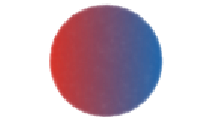
\includegraphics[width=.19\linewidth]{figures/monge-caffarelli-nonconvex-map/mccann-t000.pdf} &
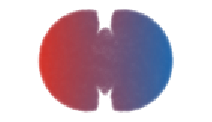
\includegraphics[width=.19\linewidth]{figures/monge-caffarelli-nonconvex-map/mccann-t025.pdf} &
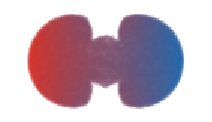
\includegraphics[width=.19\linewidth]{figures/monge-caffarelli-nonconvex-map/mccann-t050.pdf} &
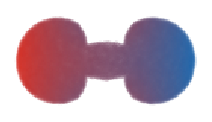
\includegraphics[width=.19\linewidth]{figures/monge-caffarelli-nonconvex-map/mccann-t075.pdf} &
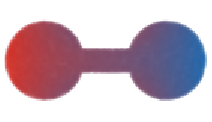
\includegraphics[width=.19\linewidth]{figures/monge-caffarelli-nonconvex-map/mccann-t100.pdf} \\[-.1em]
\small $t=0$ &
\small $t=1/4$ &
\small $t=1/2$ &
\small $t=3/4$ &
\small $t=1$
\end{tabular}
\caption{\emph{Empirical quadratic OT interpolation from a disk to a connected non-convex two-disk domain.} A \(5200\)-point farthest-point sample of the disk is matched to a \(5200\)-point farthest-point sample of two disks connected by a thin rectangle. The panels display \((1-t)x_i+tT_N(x_i)\) for the empirical optimal assignment \(T_N\). Colors are inherited from the horizontal coordinate of \(x_i\) in the initial disk, making the transported material regions visible throughout the interpolation.}
\label{fig:monge-caffarelli-nonconvex-map}
\index{Caffarelli regularity}% strictindex
\index{non-convex domain}% strictindex
\end{figure}

\begin{rem}[Regularity, weak maps, and splitting]
\index{weak!map}% strictindex
\index{splitting obstruction}% strictindex
	Caffarelli's theorem should be read as a warning as well as a theorem. Brenier's theorem gives existence and uniqueness under mild assumptions, but smoothness requires density bounds, smoothness and convex geometry that are rarely satisfied by empirical, manifold-supported or neural generative distributions. In such applications, the exact OT map is often only weakly defined, possibly unstable, and better represented by a coupling, an entropic approximation or a learned parametric surrogate.
\index{exact OT}% strictindex
\index{Brenier!theorem}% strictindex

	Even without smoothness, the convex potential is locally Lipschitz on the interior of its domain, so $\nabla\phi$ is defined Lebesgue-almost everywhere. If the source measure does not satisfy the non-splitting hypotheses of Brenier's theorem, the correct relaxed object is instead an optimal Kantorovich plan concentrated on the graph of the set-valued map $\partial\phi$. At points where $\partial\phi(x)$ contains several target locations, the plan may split the mass starting from $x$. Thus the subdifferential still describes the geometry of optimality, but the transport object is a coupling rather than a single-valued map.
\index{subdifferential}% strictindex
\index{convex!potential}% strictindex
\end{rem}

For sufficiently smooth positive densities and a classical Brenier map, the change-of-variables formula~\eqref{eq-pfwd-density} gives the Monge--Amp\`ere equation
\index{change of variables formula}% strictindex
\index{Monge-Ampere@Monge--Amp\`ere!equation}% strictindex
\eql{\label{eq-monge-ampere}
	\det(\nabla^2\phi(x))\density{\be}(\nabla\phi(x))=\density{\al}(x).
}
With suitable boundary conditions, this characterizes the Brenier potential up to an additive constant among convex solutions. The identity holds pointwise in the classical regime; for nonsmooth convex potentials it is interpreted through the Alexandrov Monge--Amp\`ere measure. The convexity constraint selects the degenerate-elliptic branch and forces $\det(\nabla^2\phi(x))\geq0$ wherever the Hessian exists.

\begin{rem}[Numerical Monge--Amp\`ere solvers]
\index{Monge-Ampere@Monge--Amp\`ere!solver}% strictindex
\index{finite difference scheme}% strictindex
\index{wide stencil}% strictindex
	The Monge--Amp\`ere operator should be viewed as a fully nonlinear, degenerate elliptic analogue of the Laplacian. Proposition~\ref{prop-linearized-monge-ampere} makes this analogy literal at first order, where the equation becomes a weighted Poisson equation. The nonlinear operator $\phi\mapsto\det(\nabla^2\phi)$, however, is elliptic only on the convex branch, together with the second boundary condition $\nabla\phi(\Omega)=\Lambda$. This is the numerical difficulty: a scheme is not reliable merely because it approximates the determinant of the Hessian. It must also select the convex Alexandrov/viscosity solution and discretize the boundary condition consistently.

	Several complementary approaches have been developed. Geometric discretizations go back to Oliker--Prussner and reflector-design methods; PDE-based solvers include Newton methods, monotone wide-stencil finite differences and variational discretizations; semi-discrete and power-diagram methods exploit the convex-cell structure of the transport map. Representative references include~\cite{oliker1989numerical,caffarelli1999problem,Loeper:2005fn,benamou2014numerical,froese2011convergent,benamou2016monotone,mirebeau2015discretization,sulman2011efficient}. We do not describe these schemes here; the point is that numerical Monge--Amp\`ere transport is primarily a problem of consistent discretization of this nonlinear Laplacian-like operator.
\index{second boundary condition}% strictindex
\index{convexity!constraint}% strictindex
\end{rem}

The following proposition records the infinitesimal form of this nonlinear equation. It is useful both conceptually and numerically: close to a smooth reference density, Monge--Amp\`ere transport reduces at first order to a weighted Poisson equation.
\index{weighted!Poisson equation}% strictindex

\begin{prop}[Linearization of the Monge--Amp\`ere equation]\label{prop-linearized-monge-ampere}
\index{Monge-Ampere@Monge--Amp\`ere!equation}% strictindex
\index{linear!linearization}% strictindex
	Let $\rho_\epsilon=\rho_0+\epsilon r+o(\epsilon)$ be a smooth perturbation of a positive reference density $\rho_0$ on a smooth bounded domain $\Omega$, with $\int_\Omega r\d x=0$. Assume that the expansions hold in a topology strong enough to differentiate the change-of-variables identity. If $\T_\epsilon(x)=x+\epsilon\nabla u(x)+o(\epsilon)$ transports $\rho_0\d x$ to $\rho_\epsilon\d x$, then, to first order,
	\[
		-\nabla\cdot(\rho_0\nabla u)=r.
	\]
	In particular, when $\rho_0$ is constant, the linearized equation is $-\Delta u=r/\rho_0$. If the source and target occupy the same fixed domain and no mass crosses its boundary, the accompanying first-order boundary condition is $\rho_0\partial_n u=0$ on $\partial\Omega$; together with $\int_\Omega u\d x=0$, it fixes the additive constant.
\end{prop}
\begin{proof}
	The change-of-variables equation for $\T_\epsilon$ is
\index{change of variables formula}% strictindex
	\[
		\rho_0(x)=\rho_\epsilon(\T_\epsilon(x))\det(\nabla \T_\epsilon(x)).
	\]
	Expanding $\rho_\epsilon(x+\epsilon\nabla u)=\rho_0(x)+\epsilon r(x)+\epsilon\dotp{\nabla\rho_0}{\nabla u}+o(\epsilon)$ and
	$\det(\Id+\epsilon\nabla^2u)=1+\epsilon\Delta u+o(\epsilon)$ gives
	\[
		\rho_0
		=
		\rho_0+
		\epsilon\bigl(r+\dotp{\nabla\rho_0}{\nabla u}+\rho_0\Delta u\bigr)+o(\epsilon)
		=
		\rho_0+
		\epsilon\bigl(r+\nabla\cdot(\rho_0\nabla u)\bigr)+o(\epsilon).
	\]
	The first-order term must vanish.
\end{proof}


%%%%%%%%%%%%%%%%%%%%%%%%%%%%%%%%%%%%%%%%%%%%%%%%%%%%%%%%%%%%%%%%%%%%%%%%%%%
\section{Beyond the Quadratic Euclidean Cost}
\index{quadratic!cost}% strictindex
\index{twist condition}% strictindex
\index{Ma-Trudinger-Wang@Ma--Trudinger--Wang condition}% strictindex
\label{sec-beyond-quadratic-euclidean-cost}

The quadratic Euclidean cost is the model case, but optimal-map theory also covers many non-quadratic costs. The key point is to separate three roles: a convexity-like structure gives potentials, a twist condition prevents splitting, and curvature-type conditions give regularity.

\paragraph{\texorpdfstring{$\Wass_p$ costs.}{Wp costs}}
\index{Wasserstein!p-distance@$p$-distance}% strictindex

The quadratic cost is special because it identifies the optimal map with the Euclidean gradient of an ordinary convex potential. For the Wasserstein cost, normalized as \(c(x,y)=\norm{x-y}^p/p\) with \(p>1\), the same Monge-map picture survives, but the potential is adapted to the cost. More generally, for \(c(x,y)=h(x-y)\) with \(h\) smooth and strictly convex, absolute continuity of the source again rules out splitting and, under the usual finite-cost assumptions, yields a unique optimal map. This map is characterized by a \(c\)-convex potential \(f\), equivalently a source-side \(\bar c\)-concave potential in the convention of Definition~\ref{def-c-concave-functions}; Section~\ref{sec-c-transfo} develops these potential classes. At differentiability points of \(f\),
\[
	\nabla f(x)=\nabla_x c(x,\T(x)).
\]
For \(c(x,y)=\norm{x-y}^p/p\), this gives the explicit relation
\[
	\T(x)=x-\norm{\nabla f(x)}^{q-2}\nabla f(x),
	\qquad \frac1p+\frac1q=1.
\]
Here $\norm{z}^{q-2}z$ denotes the continuous duality map, defined to be $0$ at $z=0$. This convention includes the case $q=2$ and removes the apparent singularity when $1<q<2$.
Thus the Brenier formula \(\T=\nabla\phi\) should be read as the quadratic representative of a broader \(c\)-convex theory. The Euclidean theory for strictly convex displacement costs is developed in Gangbo--McCann's work on the geometry of optimal transportation~\cite{gangbo1996geometry}; see also the general treatment in~\cite{Villani09}.
\index{convex!function}% strictindex
\index{Brenier!theorem}% strictindex
\index{absolute continuity}% strictindex
\index{convex!potential}% strictindex

\paragraph{Squared geodesic distance.}
\index{geodesic!distance}% strictindex
\index{Riemannian manifold}% strictindex

Let $M$ be a complete connected Riemannian manifold, let $\al,\be\in\Mm_+^1(M)$ have finite second moments, and assume that $\al$ is absolutely continuous with respect to Riemannian volume. For the squared geodesic cost \(c(x,y)=d_M(x,y)^2/2\), the Brenier--McCann theorem and its noncompact extension~\cite{mccann2001polar,FathiFigalli2010NoncompactOT} give a unique optimal map $\al$-almost everywhere. It is written with the exponential map rather than vector-space subtraction:
\[
	\T(x)=\exp_x(-\nabla\phi(x)),
\]
where \(\phi\) is \(c\)-convex and the formula is understood $\al$-almost everywhere, with $\T(x)$ outside the cut locus of $x$. This is the intrinsic version of the formula \(T=x-\nabla\phi\) in normal coordinates. The associated McCann interpolation is
\[
	\T_t(x)
	=
	\exp_x\!\left(t\exp_x^{-1}(\T(x))\right)
	=
	\exp_x(-t\nabla\phi(x)),
	\qquad
	\al_t=(\T_t)_\sharp\al,
	\qquad t\in[0,1].
\]
More generally, for an arbitrary optimal coupling $\pi$, choose a minimizing geodesic from $x$ to $y$ measurably for $\pi$-almost every $(x,y)$ and let $G_t(x,y)$ be its point at time $t$. Then $\al_t=(G_t)_\sharp\pi$. The additional issues are precisely the cut locus, possible non-uniqueness of minimizing geodesics, and regularity of the exponential map, which is why the Euclidean statement is usually presented first. These ideas feed into displacement convexity and the general manifold theory of optimal transport~\cite{mccann1997convexity,Villani09}.
\index{displacement convexity}% strictindex

Figure~\ref{fig:monge-sphere-mccann-interpolation} illustrates this intrinsic interpolation on a positively curved hemisphere.
\index{upper hemisphere}% strictindex
\index{spherical geodesic}% strictindex
\index{McCann!interpolation}% strictindex

\begin{figure}[ht]
	\centering
	
\includegraphics[width=\linewidth]{figures/monge-sphere-mccann-interpolation/evolution.pdf}
	\caption{\emph{Intrinsic McCann interpolation on the upper hemisphere.} Here \(\mathcal X=\{x\in\RR^3:\norm{x}=1,\ x_3\geq0\}\) and \(d_{\mathcal X}(x,y)=\arccos(\dotp{x}{y})\). The thin violet curves are minimizing geodesics, and the colored points show the interpolation at \(t=0,1/4,1/2,3/4,1\).}
	\label{fig:monge-sphere-mccann-interpolation}
\end{figure}

\paragraph{Poincar\'e disk.}

Negative curvature gives the complementary intrinsic interpolation shown in Figure~\ref{fig:monge-hyperbolic-mccann-interpolation}.
\index{Poincare disk@Poincar\'e disk}% strictindex
\index{hyperbolic geodesic}% strictindex
\index{McCann!interpolation}% strictindex

\begin{figure}[H]
	\centering
	
\includegraphics[width=\linewidth]{figures/monge-hyperbolic-mccann-interpolation/evolution.pdf}
	\caption{\emph{Intrinsic McCann interpolation in the Poincar\'e disk.} Here \(\mathcal X=\{x\in\RR^2:\norm{x}<1\}\) and \(d_{\mathcal X}(x,y)=\operatorname{arcosh}\!\left(1+2\norm{x-y}^2/((1-\norm{x}^2)(1-\norm{y}^2))\right)\). The black circle is the ideal boundary, the faint grid is intrinsic, and the thin violet curves are minimizing geodesics; the colored points show the interpolation at \(t=0,1/4,1/2,3/4,1\).}
	\label{fig:monge-hyperbolic-mccann-interpolation}
\end{figure}

\paragraph{Twist condition.}
\index{twist condition}% strictindex

The first non-degeneracy condition asks that the first-order information at a source point identifies at most one target point. This is the structural hypothesis that turns an optimal relation into a map.

\begin{defn}[Twist condition]\label{def-twist-condition}
	Let $X,Y\subset\RR^d$ and let $c\in C^1(X\times Y)$. The cost $c$ satisfies the twist condition from $X$ to $Y$ if, for every fixed $x\in X$, the map
	\[
		y\in Y \longmapsto \nabla_x c(x,y)\in\RR^d
	\]
	is injective. The dual twist condition is the analogous injectivity of $x\mapsto\nabla_y c(x,y)$ for every fixed $y$.
\index{dual!twist condition}% strictindex
\end{defn}

\begin{prop}[Twist prevents splitting]\label{prop-twist-prevents-splitting}
\index{twist condition}% strictindex
\index{mass!splitting}% strictindex
	Assume that $c\in C^1(X\times Y)$ satisfies the twist condition from $X$ to $Y$. Suppose that optimal pairs for the cost $c$ admit a source potential $f$ with the following first-order certificate: $f$ is differentiable on a full $\al$-measure subset of $X$, and whenever $x$ belongs to this differentiability set and $y$ can be paired optimally with $x$, one has $\nabla f(x)=\nabla_x c(x,y)$. Then, for $\al$-almost every source point $x$, there is at most one target point $y$ that can be paired optimally with $x$. Consequently, any optimal transport relation satisfying these hypotheses is single-valued $\al$-almost everywhere, hence is induced by a Monge map.
\end{prop}
\begin{proof}
	The proof uses the Kantorovich duality formalism developed later in Chapter~\ref{sec-dual}. Let $(f,g)$ be optimal Kantorovich potentials and let $\pi$ be an optimal plan. Complementary slackness gives $f(x)+g(y)=c(x,y)$ for $\pi$-almost every $(x,y)$, while dual feasibility gives $f(z)+g(y)\leq c(z,y)$ for all $z$. Thus, for almost every contact pair $(x,y)$, the function $z\mapsto c(z,y)-g(y)$ touches $f$ from above at $x$. At a point where $f$ is differentiable, this gives
	\(\nabla f(x)=\nabla_x c(x,y)\).
	If the cost is twisted, this equation determines at most one $y$. Hence no optimal plan can split the mass of such an $x$ between several target points. Since differentiability holds on a full $\al$-measure set, the plan is concentrated on the graph of a measurable map there.
\index{Kantorovich!duality}% strictindex
\index{optimal coupling}% strictindex
\index{support}% strictindex
\end{proof}

The quadratic cost satisfies twist since $\nabla_x\norm{x-y}^2=2(x-y)$; the bilinear cost $c(x,y)=-\dotp{x}{y}$ satisfies twist since $\nabla_x c(x,y)=-y$; more generally $c(x,y)=h(x-y)$ is twisted when $h$ is smooth strictly convex and $\nabla h$ is injective. On a Riemannian manifold, the squared geodesic cost is twisted locally away from the cut locus. By contrast, a separated cost $a(x)+b(y)$ is never twisted, since $\nabla_x c$ does not see $y$.
\index{cut locus}% strictindex
\index{quadratic!cost}% strictindex
\index{cost!bilinear}% strictindex
\index{strict!convexity}% strictindex

\paragraph{Ma--Trudinger--Wang curvature.}
\index{Ma-Trudinger-Wang@Ma--Trudinger--Wang condition}% strictindex
\index{Ma-Trudinger-Wang@Ma--Trudinger--Wang condition}% strictindex

Twist gives a map, but it does not by itself make this map continuous or smooth. For a general smooth cost, the relevant structural hypothesis is the Ma--Trudinger--Wang (MTW) condition, introduced for a priori estimates of the generated Jacobian equation associated with optimal transport~\cite{ma2005regularity,trudinger2001monge}.
\index{regularity theory}% strictindex
\index{Jacobian equation}% strictindex

\begin{defn}[Weak MTW condition]\label{def-mtw-condition}
\index{mixed Hessian}% strictindex
	Assume that $c\in C^4(X\times Y)$, that $X,Y\subset\RR^d$, that $c$ is twisted, and that the mixed Hessian $\nabla^2_{xy}c(x,y)$ is invertible. For $(x,p)$ in the image of the change of variables $(x,y)\mapsto(x,-\nabla_x c(x,y))$, let $Y(x,p)$ be defined by
	$-\nabla_x c(x,Y(x,p))=p$, and set
	$A_{i,j}(x,p)\eqdef-\partial^2_{x_i x_j}c(x,Y(x,p))$.
	The cost satisfies the weak MTW condition if
\index{Ma-Trudinger-Wang@Ma--Trudinger--Wang condition}% strictindex
	\[
		\sum_{i,j,k,l}\partial^2_{p_k p_l} A_{i,j}(x,p)\,\xi_i\xi_j\eta_k\eta_l\geq0
		\qquad\text{whenever }\dotp{\xi}{\eta}=0.
	\]
	A strong MTW condition asks for a positive lower bound, proportional to $\norm{\xi}^2\norm{\eta}^2$, on the same orthogonal directions.
\index{Ma-Trudinger-Wang@Ma--Trudinger--Wang condition!strong}% strictindex
\end{defn}

The tensor above is often called the cost-sectional curvature. With the sign convention used here, it measures how the negative $x$-Hessian of the cost bends when the target point is varied through the dual momentum $p$.
\index{cost-sectional curvature}% strictindex

\begin{rem}[MTW regularity landscape]\label{rem-mtw-regularity-landscape}\label{prop-mtw-regularity-implication}
\index{Ma-Trudinger-Wang@Ma--Trudinger--Wang condition}% strictindex
\index{regularity theory}% strictindex
	The regularity theorems of Ma--Trudinger--Wang, Trudinger--Wang and Loeper come in several local and global forms, with hypotheses that vary with the desired conclusion. A typical package assumes a smooth twisted and non-degenerate cost on suitable neighborhoods, mutual $c$-convexity of the domains, and source and target densities bounded above and below. Within such a package, weak MTW controls contact sets and leads to interior continuity or H\"older estimates; global boundary regularity requires additional quantitative $c$-convexity and boundary assumptions. Strong MTW, together with smoother data and domains, supports higher-order estimates for the generated Jacobian equation. These statements are a roadmap rather than a single theorem: the precise domain, density and boundary hypotheses must be taken from the corresponding result. Conversely, Loeper proved that weak MTW is necessary for continuity for arbitrary smooth positive data~\cite{ma2005regularity,trudinger2001monge,loeper2009regularity,Villani09}.
\index{Ma-Trudinger-Wang@Ma--Trudinger--Wang condition}% strictindex
\index{contact set}% strictindex
\index{c-convexity}% strictindex
\index{Jacobian equation}% strictindex
\end{rem}

The flat quadratic and bilinear costs have zero MTW curvature, hence satisfy the weak condition. For the squared Riemannian distance, the MTW tensor is a refined curvature condition on the cost: near the diagonal it recovers sectional curvature, negative sectional curvature gives an obstruction, and global regularity also depends on cut-locus and domain-convexity issues. There are nevertheless important curved examples. Round spheres have uniformly positive cost-sectional curvature away from the cut locus and satisfy the strong MTW condition~\cite{Loeper2011Sphere}; finite products of round spheres are nonnegatively cross-curved and therefore satisfy weak MTW~\cite{KimMcCann2012,FigalliKimMcCann2013}. Nonnegative cross-curvature, and hence weak MTW, is also inherited by Riemannian submersions, yielding further examples such as complex projective spaces~\cite{KimMcCann2012}. Many smooth strictly convex costs still fail MTW, which is why twist is enough for existence of a map but not for regularity.
\index{sectional curvature}% strictindex
\index{cut locus}% strictindex
\index{regularity theory}% strictindex

%%%%%%%%%%%%%%%%%%%%%%%%%%%%%%%%%%%%%%%%%%%%%%%%%%%%%%%%%%%%%%%%%%%%%%%%%%%
\section{One-Dimensional Transport and Quantiles}
\index{one-dimensional!transport}% strictindex
\index{quantile}% strictindex
\label{sec-1d-transport-quantiles}

One-dimensional OT is the model case where order replaces geometry and all constructions become explicit.

\paragraph{Cumulative and quantile functions.}
\index{cumulative distribution function}% strictindex
\index{probability integral transform}% strictindex

In one dimension, optimal transport is completely explicit. The cumulative distribution function orders the mass, and the optimal coupling is obtained by matching equal quantile levels. This special case is both a computational tool and the template for several linearized constructions used later.
\index{optimal coupling}% strictindex
\index{cumulative distribution function}% strictindex
\index{quantile!function}% strictindex

\begin{defn}[Cumulative and quantile functions]\label{def-cdf-quantile}
\index{cumulative distribution function}% strictindex
	For $\al\in\Mm_+^1(\RR)$, its cumulative distribution function is
	\eql{\label{eq-cumul-defn}
		\cumul{\al}(x)\eqdef\al((-\infty,x]).
	}
	Its generalized inverse, or quantile function, is
\index{generalized!inverse}% strictindex
	\eql{\label{eq-OT-map-1d}
		\cumul{\al}^{-1}(r)
		\eqdef
		\inf\enscond{x\in\RR}{\cumul{\al}(x)\geq r},
		\qquad r\in(0,1).
	}
\end{defn}

Figure~\ref{fig:monge-cdf-quantile-mixtures} follows three smooth laws through these representations. Their one, two, and three modes have moderately varying weights and widths. Each density mode produces a change of slope in the cumulative function, while intervals of low density become steep portions of the quantile function. The aligned quarter-mass guides make the inversion between the last two panels explicit.

\begin{figure}[H]
	\centering
	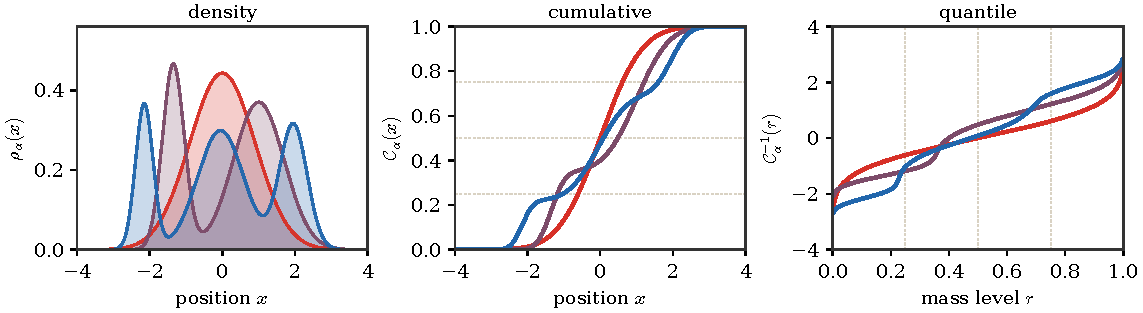
\includegraphics[width=.96\linewidth]{figures/monge-cdf-quantile-mixtures/overview.pdf}
	\caption{\emph{Densities, cumulative functions and quantiles for three Gaussian mixtures.} Transparent red, violet and blue density areas represent mixtures with one, two and three modes, respectively, with unequal component weights and widths. The cumulative functions integrate the modes into successive increases of mass, while inversion exchanges slowly varying cumulative regions with steep quantile regions. Faint guides mark the same quarter-mass levels in the last two panels.}
	\label{fig:monge-cdf-quantile-mixtures}
\end{figure}

\begin{prop}[Quantile push-forward]\label{prop-quantile-pushforward}
\index{push-forward}% strictindex
\index{quantile!push-forward}% strictindex
	One has $(\cumul{\al}^{-1})_\sharp\mathrm{Leb}_{(0,1)}=\al$. If $\al$ has no atoms, then $(\cumul{\al})_\sharp\al=\mathrm{Leb}_{(0,1)}$.
\end{prop}
\begin{proof}
	For simplicity, assume first that $\al$ has a strictly positive density, so that $\cumul{\al}$ is strictly increasing and continuous. Denote $\ga\eqdef(\cumul{\al}^{-1})_\sharp\mathrm{Leb}_{(0,1)}$. It is enough to prove that $\cumul{\ga}=\cumul{\al}$. For every $x$,
	\[
	\begin{aligned}
		\cumul{\ga}(x)
		&=
		\int_0^1 \mathbf 1_{(-\infty,x]}(\cumul{\al}^{-1}(z))\d z
		=
		\int_0^1 \mathbf 1_{[0,\cumul{\al}(x)]}(z)\d z
		=
		\cumul{\al}(x),
	\end{aligned}
	\]
	where we used $\cumul{\al}^{-1}(z)\leq x$ if and only if $z\leq\cumul{\al}(x)$. General measures follow from the same argument with generalized inverses and right-continuity of the cumulative distribution function. If $\al$ has no atoms, the probability integral transform gives $(\cumul{\al})_\sharp\al=\mathrm{Leb}_{(0,1)}$.
\index{cumulative distribution function}% strictindex
\index{generalized!inverse}% strictindex
\end{proof}

\paragraph{1D Monge solutions.}\label{par-1d-monge-solution}
\index{measure!atomless}% strictindex
\index{one-dimensional!Monge map}% strictindex
\index{Monge!problem}% strictindex

The quantile construction becomes a deterministic Monge map only when the source has no atoms, because the cumulative distribution function can then be used as a genuine change of variable. This gives an explicit one-dimensional Monge solution in the atomless case. If $\al$ has atoms, a deterministic map may fail to realize the same quantile matching because an atom cannot be split; the corresponding relaxed statement is treated in Section~\ref{sec-kantorovich-continuous}, paragraph \hyperref[sec-1d-kantorovich-solution]{Kantorovich solution in 1D}.
\index{quantile!function}% strictindex
\index{cumulative distribution function}% strictindex

\begin{thm}[One-dimensional Monge solution]\label{prop-1d-quantile-map}
\index{monotone!rearrangement}% strictindex
\index{quantile!map}% strictindex
\index{Monge!problem}% strictindex
	Let $\al,\be\in\Mm_+^1(\RR)$, assume that $\al$ has no atoms, and let $h:\RR\to[0,+\infty)$ be convex. Consider the cost $c(x,y)=h(x-y)$. Write $q_\al\eqdef\cumul{\al}^{-1}$ and $q_\be\eqdef\cumul{\be}^{-1}$, and assume that $h(q_\al-q_\be)\in L^1(0,1)$. Then
	\eql{\label{eq-1d-monge-map}
		\T=q_\be\circ\cumul{\al}
		=
		\cumul{\be}^{-1}\circ\cumul{\al}
	}
	satisfies $\T_\sharp\al=\be$ and minimizes
	\[
		\umin{S_\sharp\al=\be}\int h(x-S(x))\d\al(x).
	\]
	In particular, for any $1\leq p<+\infty$, if $\al$ and $\be$ have finite $p$th moments and $\al$ has no atoms, then $h(t)=|t|^p$ gives the usual one-dimensional Monge optimizer.
\end{thm}
\begin{proof}
	By Proposition~\ref{prop-quantile-pushforward}, atomlessness of $\al$ gives $(\cumul{\al})_\sharp\al=\mathrm{Leb}_{(0,1)}$, while $(q_\be)_\sharp\mathrm{Leb}_{(0,1)}=\be$. Hence $\T_\sharp\al=\be$.

	Let $S$ be any admissible map and set $\pi_S=(\Id,S)_\sharp\al$. The one-dimensional uncrossing theorem for relaxed couplings, proved later as Theorem~\ref{prop-1d-kantorovich-quantile-coupling}, shows that the quantile coupling $\pi^\star=(q_\al,q_\be)_\sharp\mathrm{Leb}_{(0,1)}$ is optimal among all couplings. Since $\al$ has no atoms, $(\Id,\T)_\sharp\al=\pi^\star$, and therefore
	\[
		\int h(x-\T(x))\d\al(x)
		=
		\int h(x-y)\d\pi^\star(x,y)
		\leq
		\int h(x-y)\d\pi_S(x,y)
		=
		\int h(x-S(x))\d\al(x),
	\]
	where every integral is understood in $[0,+\infty]$. This proves optimality of $\T$ among Monge maps.
\index{optimal coupling}% strictindex
\index{push-forward}% strictindex
\index{convex!function}% strictindex
\end{proof}

\begin{rem}[Composition is one-dimensional]\label{rem-1d-composition-optimal}
	In dimension one, optimal maps compose. Assume that $\al$ and $\be$ have no atoms; no atomlessness assumption is needed on $\ga$. Then the monotone rearrangements
\index{monotone!rearrangement}% strictindex
	\[
		\T_{\al\to\be}=\cumul{\be}^{-1}\circ\cumul{\al},
		\qquad
		\T_{\be\to\ga}=\cumul{\ga}^{-1}\circ\cumul{\be}
	\]
	are well defined $\al$- and $\be$-almost everywhere. Then
	\[
		\T_{\be\to\ga}\circ\T_{\al\to\be}
		=
		\T_{\al\to\ga}
		\qquad \al\text{-a.e.}
	\]
	Indeed, each map is nondecreasing and sends quantile level $r$ to the same quantile level of the target law. This semigroup property is special to the ordered line.
\end{rem}

The obstruction in higher dimension is already visible for the most elementary Gaussian maps.

\begin{example}[Linear obstruction to composing Brenier maps]
	In higher dimension, Brenier maps for the quadratic cost are gradients of convex functions, and such maps do not generally remain gradients after composition. The simplest obstruction is linear. If $\T_1(x)=A_1x$ and $\T_2(x)=A_2x$ with $A_1,A_2$ symmetric positive definite, then $\T_2\circ\T_1$ has matrix $A_2A_1$. It is a gradient field only when this product is symmetric, equivalently $A_1A_2=A_2A_1$. Gaussian transport gives a concrete instance: between nondegenerate Gaussian laws, the Brenier map is affine with symmetric positive definite linear part. Compositions of Gaussian optimal maps are therefore optimal only in special commuting situations, for instance when all covariance matrices are simultaneously diagonalizable. Otherwise the composition contains a rotational or shearing component and is not the Brenier map between the initial and final Gaussians.
\index{rotational component}% strictindex
\index{shearing component}% strictindex
\index{convex!function}% strictindex
\index{covariance!matrix}% strictindex
\index{Gaussian!optimal map}% strictindex
\index{quadratic!cost}% strictindex
\index{Brenier!map}% strictindex
\end{example}

For discrete measures, one cannot directly apply the map formula when the source has atoms, but if the measures are uniform on the same number of Dirac masses, then it is exactly the sorting formula of Proposition~\ref{prop-matching-1d-monotone}.
\index{Dirac mass}% strictindex


\begin{prop}[One-dimensional Wasserstein formulas]\label{prop-wass-quantile-1d}
\index{Wasserstein!formula}% strictindex
	Let $1\leq p<+\infty$ and let $\al,\be\in\Mm_+^1(\RR)$ have finite $p$-th moments. Then
	\eql{\label{eq-wass-cumul}
		\Wass_p(\al,\be)^p
		=
		\int_0^1\abs{\cumul{\al}^{-1}(r)-\cumul{\be}^{-1}(r)}^p\d r
		=
		\norm{\cumul{\al}^{-1}-\cumul{\be}^{-1}}_{L^p([0,1])}^p.
	}
	For $p=1$, this is equivalently
		\begin{equation}\label{eq-w1-1d}
			\Wass_1(\al,\be)
			=
			\norm{\cumul{\al}-\cumul{\be}}_{L^1(\RR)}
			=
			\int_\RR \abs{\cumul{\al}(x)-\cumul{\be}(x)}\d x
			=
			\int_\RR \abs{\int_{-\infty}^x\d(\al-\be)}\d x.
		\end{equation}
\end{prop}
\begin{proof}
	The first formula follows from Theorem~\ref{prop-1d-kantorovich-quantile-coupling}: the optimal coupling is obtained by taking the same quantile level $r$ for both measures. For $p=1$, use the layer-cake identity. If $q_\al$ and $q_\be$ are the two quantile functions, then
\index{optimal coupling}% strictindex
\index{quantile!function}% strictindex
\index{quantile!map}% strictindex
	\[
		\int_0^1 |q_\al(r)-q_\be(r)|\d r
		=
		\int_\RR
		\lambda\bigl(\{r:q_\al(r)\leq x<q_\be(r)\}\cup\{r:q_\be(r)\leq x<q_\al(r)\}\bigr)\d x.
	\]
	The measure of the displayed set is exactly $|\cumul{\al}(x)-\cumul{\be}(x)|$ for almost every $x$.
\end{proof}

For $p=2$, Bobkov and Ledoux~\cite{BobkovLedoux2019EmpiricalKantorovich} record a complementary representation involving only cumulative distribution functions, communicated to them by E.~del Barrio. It gives the same exact value as the quantile formula, but replaces the inverse-CDF step by an integral over CDF values. This is useful when cumulative functions are easier to estimate or aggregate than quantiles. This cumulative formula has recently been used to design data-parallel estimators of sliced Wasserstein distances~\cite{VauthierMerigotKorba2026CDFSW}.

\begin{prop}[Bobkov--Ledoux cumulative formula]\label{prop-bobkov-ledoux-cdf-w2}
\index{Bobkov-Ledoux@Bobkov--Ledoux formula}% strictindex
\index{CDF formula}% strictindex
\index{cumulative distribution function}% strictindex
\index{Wasserstein!formula}% strictindex
	Let $\al,\be\in\Mm_+^1([a,b])$ and write $s_+\eqdef\max(s,0)$. Then
	\eql{\label{eq-bobkov-ledoux-cdf-w2}
		\Wass_2^2(\al,\be)
		=
		2\int_a^b\int_x^b
		\Big[
		\big(\cumul{\al}(x)-\cumul{\be}(y)\big)_+
		+
		\big(\cumul{\be}(x)-\cumul{\al}(y)\big)_+
		\Big]\d y\,\d x.
	}
\end{prop}
\begin{proof}
	For any $u,v\in[a,b]$, one has
	\[
		|u-v|^2
		=
		2\int_a^b\int_x^b
		\Big[
		\mathbf 1_{\{u\leq x\leq y<v\}}
		+
		\mathbf 1_{\{v\leq x\leq y<u\}}
		\Big]\d y\,\d x,
	\]
	because, when $u<v$, the integration domain is the triangle $u\leq x\leq y<v$, whose area is $(v-u)^2/2$, and the case $v<u$ is symmetric. Apply this identity with $u=q_\al(r)$ and $v=q_\be(r)$, where $q_\al=\cumul{\al}^{-1}$ and $q_\be=\cumul{\be}^{-1}$, and integrate with respect to $r\in(0,1)$. Fubini's theorem applies since the integrand is bounded. For $x\leq y$, the generalized inverse identities give, up to endpoint sets of zero Lebesgue measure,
	\[
		\lambda\enscond{r}{q_\al(r)\leq x\ \text{and}\ q_\be(r)>y}
		=
		\big(\cumul{\al}(x)-\cumul{\be}(y)\big)_+,
	\]
	and the same argument with $\al$ and $\be$ exchanged gives the second positive part.
\index{quantile!function}% strictindex
\index{layer-cake formula}% strictindex
\end{proof}

\index{sliced Wasserstein!CDF estimator}% strictindex

\begin{rem}[Quantiles linearize one-dimensional Wasserstein geometry]\label{rem-1d-wasserstein-banach-isometry}
\index{Banach-space embedding}% strictindex
\index{Hilbertian Wasserstein space}% strictindex
	Formula~\eqref{eq-wass-cumul} means that the map $\al\mapsto\cumul{\al}^{-1}$ embeds one-dimensional Wasserstein geometry isometrically into $L^p(0,1)$. Its image is the closed convex cone of almost-everywhere nondecreasing functions with finite $p$-th moment, not the whole linear space. For \(p=2\), the Wasserstein metric on probability measures over the real line is therefore Hilbertian in the precise sense of being isometric to a convex subset of a Hilbert space. This linearization explains several later simplifications: one-dimensional barycenters are averages of quantiles in Proposition~\ref{prop-quantile-barycenters}; sliced Wasserstein applies the same formula after every projection direction in Definition~\ref{def-sliced-wasserstein} and \eqref{eq-sliced-wasserstein}; the Hilbert embedding of \(\SW_2\) in Remark~\ref{rem-sliced-hilbert-embedding} collects projected quantile functions; and linear OT coordinates use a reference map to produce the Euclidean embedding \eqref{eq-lot-embedding}. The statistical formulas in Chapter~\ref{sec-statistical-ot} should also be read in this light: empirical OT on the line is the study of empirical quantile processes, while \eqref{eq-bobkov-ledoux-cdf-w2} gives an equivalent cumulative representation when inverse CDFs are inconvenient.
\end{rem}
\index{probability measure}% strictindex
\index{Wasserstein!distance}% strictindex

Figure~\ref{fig:monge-1d-quantile-geodesic} gathers the density, cumulative and quantile representations of the same one-dimensional transport problem, together with its displacement interpolation.

\begin{figure}[htbp]
\centering
\setlength{\tabcolsep}{2pt}
\begin{tabular}{@{}cccc@{}}
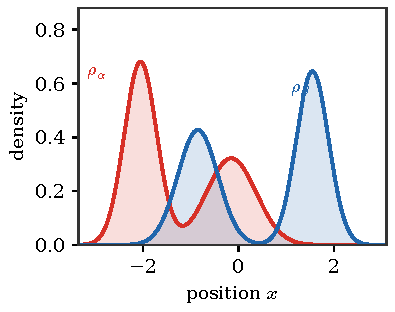
\includegraphics[width=.24\linewidth]{figures/monge-1d-quantile-geodesic/endpoint-densities.pdf} &
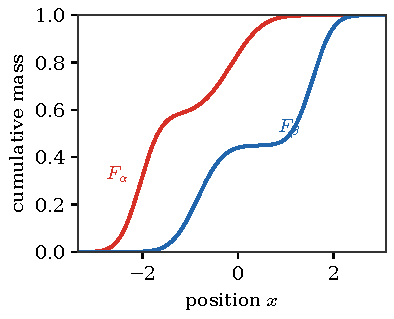
\includegraphics[width=.24\linewidth]{figures/monge-1d-quantile-geodesic/cdfs.pdf} &
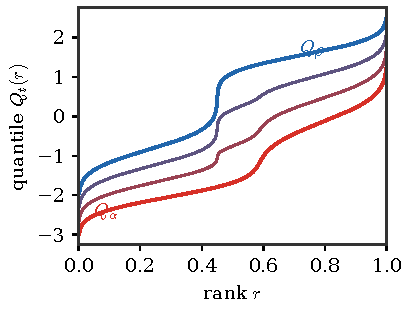
\includegraphics[width=.24\linewidth]{figures/monge-1d-quantile-geodesic/quantiles.pdf} &
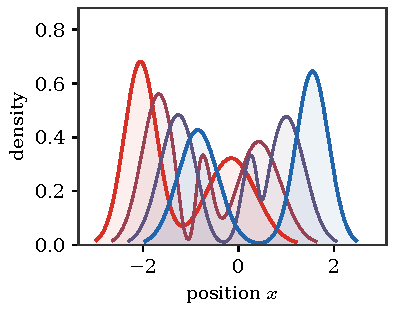
\includegraphics[width=.24\linewidth]{figures/monge-1d-quantile-geodesic/geodesic-densities.pdf} \\[-.1em]
\small densities &
\small cumulative functions &
\small quantiles &
\small displacement geodesic
\end{tabular}
\caption{\emph{One-dimensional transport through quantiles.} The same two smooth laws are shown as densities, cumulative functions and quantile functions. The last panel displays the displacement interpolation obtained by the linear quantile path $Q_t=(1-t)Q_\alpha+tQ_\beta$, which is the explicit one-dimensional $\Wass_2$ geodesic.}
\index{one-dimensional!transport}% strictindex
\index{displacement interpolation}% strictindex
\index{quantile!function}% strictindex
\label{fig:monge-1d-quantile-geodesic}
\end{figure}

The last panel is the one-dimensional specialization of the displacement interpolation of Section~\ref{sec-monge-interpolation}. In quantile coordinates, the interpolating measure is characterized by
\index{Monge!interpolation}% strictindex
\[
	\cumul{\al_t}^{-1}(r)
	=
	(1-t)\cumul{\al}^{-1}(r)+t\cumul{\be}^{-1}(r),
	\qquad r\in(0,1).
\]
The histogram-equalization figure in Section~\ref{sec-monge-pbm} is the same construction applied to pixel intensities.
\index{histogram}% strictindex

\begin{rem}[$\Wass_1$ is a norm]\label{rem-w1-norm-1d}
	For a finite signed measure $\xi$ on $\RR$ with $\xi(\RR)=0$, define its cumulative primitive by $F_\xi(x)=\xi((-\infty,x])$. Then
	\[
		\norm{\xi}_{\Wass_1}\eqdef\int_\RR|F_\xi(x)|\d x
	\]
	is a norm on the vector space of such measures satisfying $F_\xi\in L^1(\RR)$. Indeed, linearity of $\xi\mapsto F_\xi$ gives homogeneity and the triangle inequality. If $F_\xi=0$ almost everywhere, its right-continuity gives $F_\xi=0$ everywhere; hence $\xi((a,b])=F_\xi(b)-F_\xi(a)=0$ for every $a<b$, and therefore $\xi=0$. For $\xi=\al-\be$ with $\al,\be$ of finite first moment, Formula~\eqref{eq-w1-1d} identifies this norm with $\Wass_1(\al,\be)$. The condition $\int_\RR |x|\d|\xi|(x)<+\infty$ is sufficient but not necessary for finiteness. More generally, Kantorovich--Rubinstein duality defines an analogous norm on every metric space on its finite domain; see Section~\ref{sec-W1}. What is special to the line is this explicit primitive representation.
\end{rem}

\paragraph{Norms on cumulative functions.}
The identity~\eqref{eq-w1-1d} singles out the $L^1$ norm of cumulative functions. Replacing it by another $L^p$ norm produces a useful family of one-dimensional discrepancies.

\begin{defn}[Cumulative-function distances]\label{def-cumulative-function-distance}
\index{cumulative distribution function!distance}% strictindex
	For $\al,\be\in\Mm_+^1(\RR)$ and $1\leq p<+\infty$, define
	\eql{\label{eq-cumulative-function-distance}
		D_p(\al,\be)
		\eqdef
		\norm{\cumul{\al}-\cumul{\be}}_{L^p(\RR)}.
	}
	The endpoint distance is
	\eq{
		D_\infty(\al,\be)
		\eqdef
		\sup_{x\in\RR}\abs{\cumul{\al}(x)-\cumul{\be}(x)}.
	}
\end{defn}

Minkowski's inequality gives the triangle inequality, while two right-continuous cumulative functions that agree almost everywhere agree everywhere. Thus $D_p$ is an extended metric. Since $\abs{\cumul{\al}-\cumul{\be}}\leq1$, one has $D_p^p\leq D_1=\Wass_1$, so it is finite whenever the measures have finite first moments. In classical terminology, $D_1$ is exactly $\Wass_1$, $D_2$ is the Cram\'er distance, and $D_\infty$ is the Kolmogorov--Smirnov distance. The following proposition makes precise how the finite-$p$ distances compare with Wasserstein geometry.
\index{cumulative distribution function!norm}% strictindex
\index{Cramer distance@Cram\'er distance}% strictindex
\index{Kolmogorov-Smirnov@Kolmogorov--Smirnov distance}% strictindex

\begin{prop}[Cumulative-function and Wasserstein distances]\label{prop-cumulative-wasserstein-comparison}
	Let $1\leq p<+\infty$ and let $\al,\be\in\Mm_+^1(\RR)$ have finite $p$th moments. Then
	\eql{\label{eq-cumulative-wasserstein-global-comparison}
		D_p(\al,\be)^p
		\leq
		D_1(\al,\be)
		=
		\Wass_1(\al,\be)
		\leq
		\Wass_p(\al,\be).
	}
	If $\supp(\al)\cup\supp(\be)$ is contained in an interval of length $L>0$, then
	\eql{\label{eq-cumulative-wasserstein-bounded-comparison}
		\left(\frac{D_p(\al,\be)}{L^{1/p}}\right)^p
		\leq
		\frac{\Wass_p(\al,\be)}{L}
		\leq
		\left(\frac{D_p(\al,\be)}{L^{1/p}}\right)^{1/p}.
	}
	For the endpoint CDF metric $D_\infty$, every $1\leq r<+\infty$ satisfies
	\eq{
		\Wass_r(\al,\be)
		\leq
		L D_\infty(\al,\be)^{1/r}.
	}
\end{prop}
\begin{proof}
	Set $h=\cumul{\al}-\cumul{\be}$. Since $\abs{h}\leq1$, one has $\int_\RR\abs{h}^p\leq\int_\RR\abs{h}$. Formula~\eqref{eq-w1-1d} identifies the latter integral with $\Wass_1(\al,\be)$. Moreover, for every $\pi\in\Couplings(\al,\be)$,
	\eq{
		\Wass_1(\al,\be)
		\leq \int_{\RR^2}\abs{x-y}\d\pi(x,y)
		\leq \left(\int_{\RR^2}\abs{x-y}^p\d\pi(x,y)\right)^{1/p}.
	}
	Taking the infimum over $\pi$ proves~\eqref{eq-cumulative-wasserstein-global-comparison}.

	Under the support assumption, $h$ vanishes outside an interval of length $L$, so H\"older's inequality gives
	$\Wass_1(\al,\be)\leq L^{1-1/p}D_p(\al,\be)$. The common quantile coupling is optimal for every Wasserstein exponent by Proposition~\ref{prop-wass-quantile-1d}, and all its displacements have magnitude at most $L$. Evaluating its $p$-cost therefore gives
	\eq{
		\Wass_p(\al,\be)^p
		\leq L^{p-1}\Wass_1(\al,\be)
		\leq L^{p-1/p}D_p(\al,\be).
	}
	Taking the $p$th root and dividing by $L$ proves the upper bound in~\eqref{eq-cumulative-wasserstein-bounded-comparison}; its lower bound follows from~\eqref{eq-cumulative-wasserstein-global-comparison}. Finally, $\Wass_1(\al,\be)\leq L D_\infty(\al,\be)$ and the same bounded-displacement argument gives $\Wass_r(\al,\be)^r\leq L^{r-1}\Wass_1(\al,\be)$, proving the endpoint estimate.
\end{proof}

\Needspace{6\baselineskip}
For $p=1$, the inequalities collapse to the already known identity $D_1=\Wass_1$. For every $1\leq p<+\infty$, the two-sided H\"older estimate~\eqref{eq-cumulative-wasserstein-bounded-comparison} shows that $D_p$ and $\Wass_p$ induce the same topology on laws supported in a fixed compact interval. By Proposition~\ref{prop-wass-topology-polish}, this common topology is weak convergence.

On the whole line, among laws with finite $p$th moment, the $\Wass_p$ topology is stronger by~\eqref{eq-cumulative-wasserstein-global-comparison}, and it is strictly stronger when $p>1$. Indeed, for $\al=\de_0$ and $\be_n=(1-n^{-1})\de_0+n^{-1}\de_n$, one has $D_p(\al,\be_n)^p=n^{1-p}\to0$, whereas $\Wass_p(\al,\be_n)^p=n^{p-1}\to+\infty$.

The endpoint $p=\infty$ should not be included in the compact-support equivalence. Even on $[0,1]$, $D_\infty$ and $\Wass_\infty$ are topologically incomparable: $\Wass_\infty(\de_{1/n},\de_0)=n^{-1}$ while $D_\infty(\de_{1/n},\de_0)=1$, whereas for $\widetilde\be_n=(1-n^{-1})\de_0+n^{-1}\de_1$ one has $D_\infty(\widetilde\be_n,\de_0)=n^{-1}$ but $\Wass_\infty(\widetilde\be_n,\de_0)=1$.
\index{convergence!in law}% strictindex
\index{topology!cumulative-distribution-function distance}% strictindex
\index{signed!measure}% strictindex
\index{Kantorovich-Rubinstein@Kantorovich--Rubinstein!norm}% strictindex

\paragraph{OT on trees.}
\index{OT on trees}% strictindex
\index{tree!transport}% strictindex
\index{edge imbalance}% strictindex
\index{tree!metric}% strictindex

The line is the simplest tree. On a general tree, the order is no longer total, but each edge still defines a cut and hence a cumulative imbalance. This gives an exact formula for the $\Wass_1$ cost associated with the tree geodesic distance. The formula is classical in fast earth-mover computations on tree metrics~\cite{TreeEMD2007} and is also the mechanism behind tree-sliced Wasserstein distances~\cite{LeYamadaFukumizuCuturi2019TreeSliced}.
\index{tree-Wasserstein distance}% strictindex
\index{tree!earth mover distance}% strictindex

\begin{prop}[Cumulative formula on a tree]\label{prop-tree-w1-cumulative}
	Let $\mathsf{T}=(V,E,\ell)$ be a finite weighted tree, where each edge $e$ has length $\ell_e>0$, and let $d_{\mathsf{T}}$ be its geodesic distance. Choose a root $o$. For an edge $e=(u,v)$ oriented away from $o$, let $V_e$ be the set of vertices in the connected component containing $v$ after removing $e$. If $\al,\be\in\Pp(V)$, then
	\eql{\label{eq-tree-w1-cumulative}
		\Wass_{1,d_{\mathsf{T}}}(\al,\be)
		=
		\umin{\pi\in\Couplings(\al,\be)}
		\sum_{x,y\in V} d_{\mathsf{T}}(x,y)\pi_{x y}
		=
		\sum_{e\in E}\ell_e
		\abs{\al(V_e)-\be(V_e)}.
	}
	The value is computable in $O(|V|)$ arithmetic operations once the signed masses $\al-\be$ are stored on the vertices, by one postorder traversal of the rooted tree.
\end{prop}
\begin{proof}
	Let $\sigma=\al-\be$. Removing an edge $e$ splits the tree into $V_e$ and its complement. For any coupling $\pi$, the net amount of mass crossing $e$ from $V_e$ to $V\setminus V_e$ minus the amount crossing in the reverse direction is fixed and equals $\sigma(V_e)$. Hence the total amount of transported mass whose path uses $e$ is at least $|\sigma(V_e)|$. Since every unit of mass crossing $e$ pays the length $\ell_e$, summing over edges gives
	\[
		\sum_{x,y}d_{\mathsf{T}}(x,y)\pi_{x,y}
		=
		\sum_{e\in E}\ell_e
		\sum_{x,y:\ e\in[x,y]}\pi_{x,y}
		\geq
		\sum_{e\in E}\ell_e|\sigma(V_e)|,
	\]
	where $[x,y]$ is the unique path between $x$ and $y$.

	It remains to realize this lower bound. Process the rooted tree from the leaves to the root. At a vertex $v\neq o$, compute the total signed mass in the subtree below $v$, namely $F_e=\sigma(V_e)$ for the edge $e$ joining $v$ to its parent. If $F_e>0$, send $F_e$ units of surplus from this subtree to the parent side; if $F_e<0$, import $-F_e$ units from the parent side into the subtree. After this operation the subtree has zero net imbalance and can be collapsed into its parent. Continuing upward balances all subtrees because $\sigma(V)=0$. Decomposing these edge fluxes into source-to-target paths yields a coupling whose traffic across each edge is exactly $|F_e|$, and therefore whose cost is the right-hand side of~\eqref{eq-tree-w1-cumulative}. The same postorder pass computes all $F_e$, proving the complexity claim.
\end{proof}

For a chain rooted at one end, the sets $V_e$ are rays, so~\eqref{eq-tree-w1-cumulative} is the discrete version of the one-dimensional identity~\eqref{eq-w1-1d}. This edgewise cumulative decoupling is specific to the geodesic-distance cost $d_{\mathsf{T}}$, i.e.\ to $\Wass_1$. For powers $d_{\mathsf{T}}^p$ with $p>1$, the term $\big(\sum_{e\in[x,y]}\ell_e\big)^p$ couples all edges along a path, so the simple sum of absolute subtree imbalances no longer gives the optimal value. The tree structure remains algorithmically useful in a different sense: tree metrics give fast surrogates and embeddings for EMD-type computations on histograms~\cite{indyk,andoni2008earth,TreeEMD2007}, and randomized or data-adapted trees lead to tree-sliced Wasserstein distances that trade the exact Euclidean ground metric for much faster one-dimensional/tree computations~\cite{LeYamadaFukumizuCuturi2019TreeSliced}.
\index{tree!embedding}% strictindex
\index{tree-sliced Wasserstein}% strictindex
\index{cumulative distribution function}% strictindex
\index{geodesic!distance}% strictindex

The same tree can nevertheless be used as a genuine geodesic space. If $\pi$ is an optimal coupling for the squared tree distance $d_{\mathsf{T}}^2$, the associated displacement interpolation moves each packet of mass $\pi_{i,j}$ at constant speed along the unique path from $x_i$ to $x_j$. Figure~\ref{fig:monge-tree-mccann-interpolation} shows this tree analogue of McCann interpolation. The intermediate measures are not necessarily supported on the original vertices: mass may sit inside edges while it travels through the branching structure.
\index{McCann!interpolation}% strictindex
\index{tree!geodesic}% strictindex

\begin{figure}[htbp]
\centering
\setlength{\tabcolsep}{1.5pt}
\begin{tabular}{@{}ccccc@{}}

\includegraphics[width=.19\linewidth]{figures/monge-tree-mccann-interpolation/time-000.pdf} &

\includegraphics[width=.19\linewidth]{figures/monge-tree-mccann-interpolation/time-025.pdf} &

\includegraphics[width=.19\linewidth]{figures/monge-tree-mccann-interpolation/time-050.pdf} &

\includegraphics[width=.19\linewidth]{figures/monge-tree-mccann-interpolation/time-075.pdf} &

\includegraphics[width=.19\linewidth]{figures/monge-tree-mccann-interpolation/time-100.pdf} \\[-.1em]
\small $t=0$ &
\small $t=.25$ &
\small $t=.5$ &
\small $t=.75$ &
\small $t=1$
\end{tabular}
\caption{\emph{McCann interpolation on a finite tree.} A quadratic optimal plan is computed between two non-uniform vertex histograms for the squared geodesic distance on the tree. Each transported packet then moves along the unique tree path connecting its source and target vertices. Circle areas encode transported masses, colors interpolate from the source measure $\al$ in red to the target measure $\be$ in blue, and faint colored corridors mark the tree branches carrying transport.}
\index{tree!interpolation}% strictindex
\index{displacement interpolation}% strictindex
\label{fig:monge-tree-mccann-interpolation}
\end{figure}

\paragraph{Triangular rearrangements.}
\index{triangular rearrangement}% strictindex

There is another canonical way to build transport maps in several dimensions: transport one coordinate at a time by conditional one-dimensional quantiles. This construction goes back to Knothe and Rosenblatt~\cite{Knothe1957,Rosenblatt1952}. It is not usually cost-optimal, but it gives a deterministic rearrangement under weak assumptions and clarifies how multivariate transport can be reduced recursively to scalar monotone maps.
\index{transport!map}% strictindex

\begin{prop}[Knothe--Rosenblatt triangular rearrangement]\label{prop-knothe-rosenblatt}
\index{Knothe-Rosenblatt rearrangement@Knothe--Rosenblatt rearrangement}% strictindex
	Let $\al,\be\in\Mm_+^1(\RR^d)$. Assume that the first marginal of $\al$ and, recursively, the one-dimensional conditional source laws used below are atomless almost everywhere. Fix measurable versions of all regular conditional distributions. Then there is a triangular map
\index{regular conditional distribution}% strictindex
\index{conditional!law}% strictindex
\index{triangular map}% strictindex
	\[
		\T(x_1,\ldots,x_d)
		=
		(\T_1(x_1),\T_2(x_1,x_2),\ldots,\T_d(x_1,\ldots,x_d))
	\]
	such that $\T_\sharp\al=\be$ and, for each $k$, the function $x_k\mapsto\T_k(x_1,\ldots,x_k)$ is nondecreasing for $\al_{<k}$-almost every $x_{<k}=(x_1,\ldots,x_{k-1})$.
\end{prop}
\begin{proof}
	The construction is recursive. For $k=1$, let $\T_1$ be the monotone rearrangement between the first marginal of $\al$ and the first marginal of $\be$. Suppose that $\T_1,\ldots,\T_{k-1}$ have already been constructed. Write $x_{<k}=(x_1,\ldots,x_{k-1})$ and $\T_{<k}=(\T_1,\ldots,\T_{k-1})$. By induction, $(\T_{<k})_\sharp\al_{<k}=\be_{<k}$, where $\al_{<k}$ and $\be_{<k}$ are the first $(k-1)$-coordinate marginals. Let $\al^k_{x_{<k}}$ and $\be^k_{y_{<k}}$ be regular conditional laws of the $k$-th coordinate given the previous coordinates. Define $\T_k(x_{<k},\cdot)$ as the one-dimensional monotone rearrangement from $\al^k_{x_{<k}}$ to $\be^k_{\T_{<k}(x_{<k})}$.
\index{monotone!rearrangement}% strictindex

	The map $\T_k(x_{<k},\cdot)$ is nondecreasing by the one-dimensional rearrangement theorem. The chain rule for disintegrations then shows that, after step $k$, the first $k$ coordinates of $\T_\sharp\al$ have the same law as the first $k$ coordinates of $\be$. At $k=d$ this gives $\T_\sharp\al=\be$. Target atoms are handled by generalized quantiles. If a source conditional law has atoms that must be split, the same recursive construction defines a triangular Markov kernel rather than a deterministic map.
\index{disintegration}% strictindex
\index{Markov kernel}% strictindex
\index{generalized quantile}% strictindex
\index{conditional!law}% strictindex
\end{proof}

The recursive construction in the proof is an algorithm: it repeatedly applies the one-dimensional quantile rearrangement to conditional distributions.

\begin{alg}[Knothe--Rosenblatt triangular rearrangement]\label{alg:triangular-rearrangement}
\index{Knothe-Rosenblatt rearrangement@Knothe--Rosenblatt rearrangement}% strictindex
\textbf{Input:} Probability measures $\al,\be$ on $\RR^d$ with regular conditional laws, with every source conditional law used below atomless.

\textbf{Output:} Knothe--Rosenblatt triangular map $\T$.

\textbf{Compute} first-coordinate rearrangement:
\(\T_1=(F_{\be_1})^{-1}\circ F_{\al_1}\).

\textbf{For} $k=2,\ldots,d$ \textbf{do}:
\begin{algblock}

\textbf{Set} $x_{<k}=(x_1,\ldots,x_{k-1})$.

\textbf{Compute} conditional laws $\al^k_{x_{<k}}$ and $\be^k_{\T_{<k}(x_{<k})}$.

\textbf{Set}
\(\T_k(x_{<k},x_k) = \bigl(F_{\be^k_{\T_{<k}(x_{<k})}}\bigr)^{-1} \circ F_{\al^k_{x_{<k}}}(x_k)\).
\end{algblock}
\algreturnskip
\textbf{Return} \(\T(x)=(\T_1(x_1),\T_2(x_1,x_2),\ldots,\T_d(x_1,\ldots,x_d))\).
\end{alg}

Figure~\ref{fig:monge-triangular-rearrangement} shows the two-dimensional mechanism on image histograms. The first stage transports only the horizontal marginal, so the middle pivot has the same $x$-marginal as the target but keeps the source vertical conditionals. The second stage then transports each vertical conditional law inside the corresponding column.
\index{histogram}% strictindex
\index{conditional!law}% strictindex
\index{triangular rearrangement}% strictindex

\begin{figure}[H]
\centering
\setlength{\tabcolsep}{1pt}
\begin{tabular}{@{}ccccccc@{}}
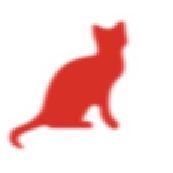
\includegraphics[width=.135\linewidth]{figures/monge-triangular-rearrangement/stage-01-source.pdf} &

\includegraphics[width=.135\linewidth]{figures/monge-triangular-rearrangement/stage-02-horizontal-033.pdf} &
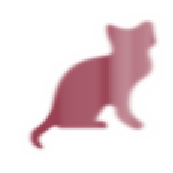
\includegraphics[width=.135\linewidth]{figures/monge-triangular-rearrangement/stage-03-horizontal-067.pdf} &
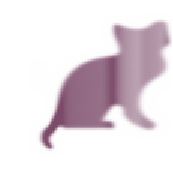
\includegraphics[width=.135\linewidth]{figures/monge-triangular-rearrangement/stage-04-pivot.pdf} &
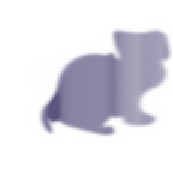
\includegraphics[width=.135\linewidth]{figures/monge-triangular-rearrangement/stage-05-vertical-033.pdf} &
\index{triangular rearrangement}% strictindex
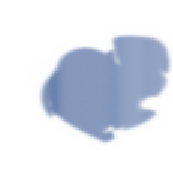
\includegraphics[width=.135\linewidth]{figures/monge-triangular-rearrangement/stage-06-vertical-067.pdf} &
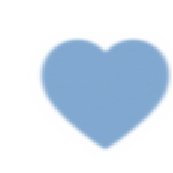
\includegraphics[width=.135\linewidth]{figures/monge-triangular-rearrangement/stage-07-target.pdf} \\[-.1em]
\small source &
\small $x$-move &
\small $x$-move &
\small pivot &
\small $y$-move &
\small $y$-move &
\small target
\end{tabular}
\caption{\emph{Triangular rearrangement between the same cat and heart densities as in Figure~\ref{fig:monge-shape-mccann-interpolation}.} The panels are computed directly on image histograms. The first three transitions move mass horizontally by the monotone rearrangement between the $x$-marginals; the pivot has the target horizontal marginal. The last three transitions keep each column fixed and move mass vertically by one-dimensional monotone rearrangements between conditional laws.}
\index{triangular rearrangement}% strictindex
\index{monotone!rearrangement}% strictindex
\index{McCann!interpolation}% strictindex
\label{fig:monge-triangular-rearrangement}
\end{figure}

This construction transports successively along coordinate axes and is therefore often called axis-wise transport. It depends on the chosen ordering of coordinates and is not generally optimal for the quadratic cost. It is nevertheless a useful limiting object: Brenier maps for increasingly anisotropic quadratic costs converge to triangular rearrangements under suitable assumptions~\cite{carlier2010knothe}.
\index{quadratic!cost}% strictindex
\index{Brenier!map}% strictindex
\index{triangular rearrangement}% strictindex

\begin{prop}[Anisotropic Brenier maps converge to Knothe--Rosenblatt]\label{prop-knothe-limit-anisotropic-brenier}
\index{Knothe-Rosenblatt rearrangement@Knothe--Rosenblatt rearrangement}% strictindex
	Let $\al,\be$ be compactly supported probability measures on $\RR^d$ with densities bounded above and below on their rectangular supports. In particular, the source and target conditional laws entering the Knothe--Rosenblatt construction are atomless almost everywhere. For $\epsilon>0$, set
\index{conditional!law}% strictindex
\index{probability measure}% strictindex
	\[
		c_\epsilon(x,y)
		\eqdef
		\sum_{k=1}^d \epsilon^{k-1}\abs{x_k-y_k}^2.
	\]
	Let $T_\epsilon$ be the Monge map from $\al$ to $\be$ for the cost $c_\epsilon$, and let $T_{\mathrm{KR}}$ be the triangular Knothe--Rosenblatt rearrangement with the coordinate order used above. Then
\index{Monge!problem}% strictindex
\index{Knothe-Rosenblatt rearrangement@Knothe--Rosenblatt rearrangement}% strictindex
	\[
		T_\epsilon \longrightarrow T_{\mathrm{KR}}
		\qquad\text{in } L^2(\al;\RR^d)
		\qquad\text{as } \epsilon\to0.
	\]
\end{prop}

\begin{proof}
		We summarize the scale-separated argument of~\cite{carlier2010knothe}. Let $\pi_\epsilon=(\Id,T_\epsilon)_\sharp\al$. For a coupling $\gamma$, set $I_k(\gamma)\eqdef\int\abs{x_k-y_k}^2\d\gamma(x,y)$ and $F_\epsilon(\gamma)\eqdef\sum_{k=1}^d\epsilon^{k-1}I_k(\gamma)$.
	Since the supports are compact, every sequence $\epsilon\downarrow0$ has a subsequence for which $\pi_\epsilon$ converges weakly to a coupling $\pi$ between $\al$ and $\be$. The coordinate costs are bounded and continuous on the common compact support. Dividing $F_\epsilon$ by its leading coefficient and passing to the limit shows that $\pi$ minimizes $I_1$. The first source marginal is atomless, so the $(x_1,y_1)$-marginal of $\pi$ is the unique monotone coupling; equivalently, $y_1=T_1(x_1)$ under $\pi$.
\index{monotone!rearrangement}% strictindex
\index{quadratic!cost}% strictindex

	The next scale identifies the second coordinate. Optimality against the Knothe coupling $\pi_{\mathrm{KR}}$ gives $F_\epsilon(\pi_\epsilon)\leq F_\epsilon(\pi_{\mathrm{KR}})$. Since $I_1(\pi_\epsilon)$ is bounded below by the optimal first-coordinate value $I_1(\pi_{\mathrm{KR}})$, cancellation and division by $\epsilon$ yield
	\[
		\sum_{k=2}^d\epsilon^{k-2}I_k(\pi_\epsilon)
		\leq\sum_{k=2}^d\epsilon^{k-2}I_k(\pi_{\mathrm{KR}}).
	\]
	Passing to the limit shows that $\pi$ minimizes $I_2$ among couplings with the already identified first-coordinate marginal. Disintegration with respect to $(x_1,y_1)$ turns this into the monotone transport between the conditional laws of $x_2$ and $y_2$, so $y_2=T_2(x_1,x_2)$ under $\pi$.
\index{conditional!law}% strictindex

	The higher-coordinate induction repeats this comparison after disintegrating over the already identified coordinates. Its technical point is to control the residual suboptimality of the earlier coordinates before dividing by the next power of $\epsilon$; the atomlessness of both source and target conditionals makes the preceding monotone couplings invertible almost everywhere. The scale-separated estimate proved in~\cite{carlier2010knothe} then gives successively $y_k=T_k(x_1,\ldots,x_k)$ for every $k$. Consequently, every weak limit is the graph coupling $\pi_{\mathrm{KR}}=(\Id,T_{\mathrm{KR}})_\sharp\al$, and uniqueness of this limit gives convergence of the whole family.
\index{weak!limit}% strictindex

	Finally, let $X\sim\al$. The graph couplings are the laws of $(X,T_\epsilon(X))$, and they converge weakly to the law of $(X,T_{\mathrm{KR}}(X))$. To turn this into convergence of maps, fix $\zeta>0$. By Lusin's theorem, there is a compact set $K$ with $\al(K)>1-\zeta$ on which $T_{\mathrm{KR}}$ is continuous. On $K$, the set
	\[
		\enscond{(x,y)}{x\in K,\ \norm{y-T_{\mathrm{KR}}(x)}\geq\delta}
	\]
	is closed and has zero mass under the limiting graph coupling. Portmanteau's theorem gives
\index{zero mass}% strictindex
	\[
		\limsup_{\epsilon\to0}
		\al\!\left(\enscond{x}{x\in K,\ \norm{T_\epsilon(x)-T_{\mathrm{KR}}(x)}\geq\delta}\right)
		=0.
	\]
	Adding the complement of $K$ and letting $\zeta\to0$ proves convergence in $\al$-probability. Since all maps take values in a common compact set, their squared differences are uniformly integrable, and convergence therefore holds in $L^2(\al)$.
\end{proof}

%%%%%%%%%%%%%%%%%%%%%%%%%%%%%%%%%%%%%%%%%%%%%%%%%%%%%%%%%%%%%%%%%%%%%%%%%%%
\section{Gaussian Measures and the Bures Metric}
\index{Gaussian!measure}% strictindex
\index{Bures!metric}% strictindex
\label{sec-gaussian-bures}

Gaussian measures form the most important finite-dimensional family preserved by quadratic optimal transport. The mean moves linearly, while the covariance follows the Bures--Wasserstein geometry of positive semidefinite matrices.
\index{positive!semidefinite matrix}% strictindex
\index{Bures!Wasserstein geometry}% strictindex

\paragraph{One-dimensional Gaussians.}
\index{Gaussian!measure}% strictindex

Let $\al=\Gaussian(m_\al,\sigma_\al^2)$ and $\be=\Gaussian(m_\be,\sigma_\be^2)$ be two nondegenerate Gaussians on $\RR$. Then
\[
	\T(x)=\frac{\sigma_\be}{\sigma_\al}(x-m_\al)+m_\be
\]
satisfies $\T_\sharp\al=\be$. It is the derivative of the convex function
\index{convex!function}% strictindex
\[
	\phi(x)=\frac{\sigma_\be}{2\sigma_\al}(x-m_\al)^2+m_\be x,
\]
so Brenier's theorem shows that it is the optimal quadratic transport. The associated distance is
\index{Brenier!theorem}% strictindex
\[
	\Wass_2(\al,\be)^2
	=
	\int_\RR\left(\frac{\sigma_\be}{\sigma_\al}(x-m_\al)+m_\be-x\right)^2\d\al(x)
	=
	(m_\al-m_\be)^2+(\sigma_\al-\sigma_\be)^2.
\]
The formula extends by continuity to Dirac masses, although the affine Monge map itself only pushes a Dirac source to another Dirac. Thus the OT geometry of one-dimensional Gaussians is the Euclidean geometry of the closed half-plane $(m,\sigma)\in\RR\times\RR_+$. By contrast, the Fisher--Rao boundary $\sigma=0$ is infinitely far from every nondegenerate Gaussian, and the KL divergence from a nondegenerate Gaussian to a singular one is infinite.
\index{Monge!problem}% strictindex
\index{Dirac mass}% strictindex
\index{Gaussian!measure}% strictindex

Figure~\ref{fig:monge-gaussian-w2-geodesic-1d} displays this Euclidean half-plane geometry and the corresponding displacement interpolation of the Gaussian densities.

\begin{figure}[htbp]
\centering
\setlength{\tabcolsep}{2pt}
\begin{tabular}{@{}ccc@{}}
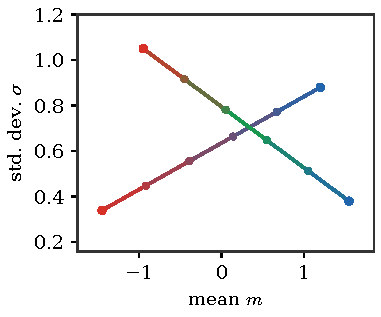
\includegraphics[width=.30\linewidth]{figures/monge-gaussian-w2-geodesic/halfplane-1d.pdf} &
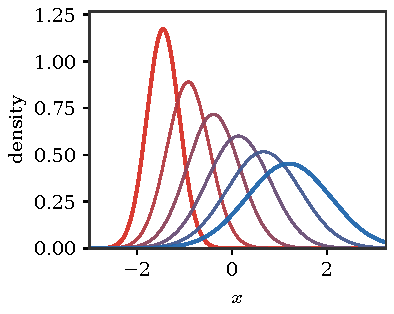
\includegraphics[width=.32\linewidth]{figures/monge-gaussian-w2-geodesic/densities-1d-a.pdf} &
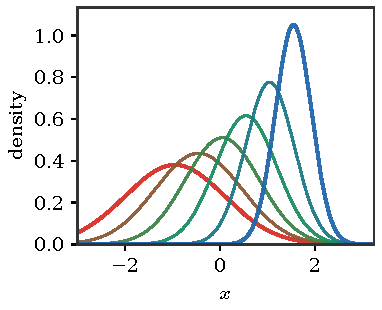
\includegraphics[width=.32\linewidth]{figures/monge-gaussian-w2-geodesic/densities-1d-b.pdf} \\[-.1em]
\small $(m,\sigma)$ half-plane &
\small first geodesic &
\small second geodesic
\end{tabular}
\caption{\emph{One-dimensional Gaussian $\Wass_2$ geodesics.} In the coordinates $(m,\sigma)$, the geodesics are Euclidean segments in the upper half-plane. Both paths share red and blue endpoint colors; the first interpolates directly between them, whereas the second passes through green at mid-time. The same palettes identify both segments in the left panel.}
\label{fig:monge-gaussian-w2-geodesic-1d}
\end{figure}


\begin{rem}[Comparison with the Fisher--Rao metric with mean variation]\label{rem-fisher-rao-gaussian-mean}
\index{Fisher-Rao@Fisher--Rao metric}% strictindex
\index{Gaussian!measure}% strictindex
\index{hyperbolic metric}% strictindex
\index{Kullback-Leibler@Kullback--Leibler!divergence}% strictindex
	The previous formula shows that the Wasserstein geometry of one-dimensional Gaussians is Euclidean in $(m,\sigma)$. The Fisher--Rao geometry obtained from the local expansion of the Kullback--Leibler divergence is different as soon as the mean is allowed to vary~\cite{costa2015fisher}. For $\sigma,\sigma'>0$,
	\[
		\KL\big(\Gaussian(m,\sigma^2)\mid\Gaussian(m',(\sigma')^2)\big)
		=
		\log\frac{\sigma'}{\sigma}
		+
		\frac{\sigma^2+(m-m')^2}{2(\sigma')^2}
		-
		\frac12.
	\]
	Expanding the first argument around $(m,\sigma)$ gives, for increments $(h,s)$,
	\[
		\KL\big(\Gaussian(m+\varepsilon h,(\sigma+\varepsilon s)^2)
		\mid \Gaussian(m,\sigma^2)\big)
		=
		\frac{\varepsilon^2}{2}
		\left(\frac{h^2}{\sigma^2}+2\frac{s^2}{\sigma^2}\right)
		+o(\varepsilon^2).
	\]
	Thus the Fisher--Rao metric on the Gaussian half-plane is
\index{Fisher-Rao@Fisher--Rao metric}% strictindex
	\[
		g_{(m,\sigma)}^{\mathrm{FR}}((h,s),(h',s'))
		=
		\frac{hh'+2ss'}{\sigma^2}.
	\]
	Setting $z=m/\sqrt2+i\sigma$ identifies this metric with twice the usual hyperbolic metric on the upper half-plane. Its geodesics are therefore vertical lines or Euclidean semicircles orthogonal to the boundary $\sigma=0$ after this horizontal rescaling. Consequently
	\[
		d_{\mathrm{FR}}\big(\Gaussian(m,\sigma^2),\Gaussian(m',(\sigma')^2)\big)
		=
		\sqrt2\,\operatorname{arcosh}\left(
		1+\frac{(m-m')^2+2(\sigma-\sigma')^2}{4\sigma\sigma'}
		\right).
	\]
	In contrast, $\Wass_2^2=(m-m')^2+(\sigma-\sigma')^2$. Wasserstein geodesics are straight segments in the $(m,\sigma)$ half-plane and reach $\sigma=0$ at finite distance, whereas Fisher--Rao geodesics bend away from the boundary and the boundary $\sigma=0$ is infinitely far away. Figure~\ref{fig:monge-gaussian-fr-mean-geodesic} displays the resulting difference in both parameter space and density space.
\index{Fisher-Rao@Fisher--Rao metric}% strictindex
\end{rem}

\begin{figure}[htbp]
\centering
\setlength{\tabcolsep}{2pt}
\begin{tabular}{@{}ccc@{}}
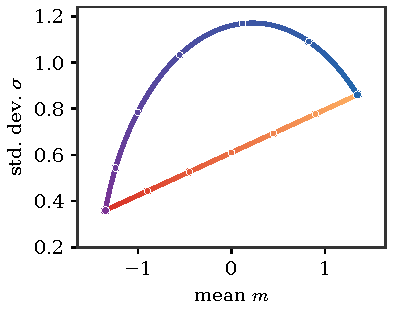
\includegraphics[width=.30\linewidth]{figures/monge-gaussian-fr-mean-geodesic/halfplane.pdf} &
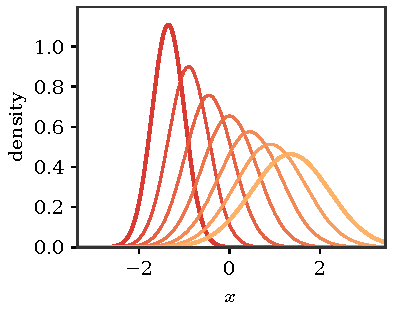
\includegraphics[width=.32\linewidth]{figures/monge-gaussian-fr-mean-geodesic/densities-w2.pdf} &
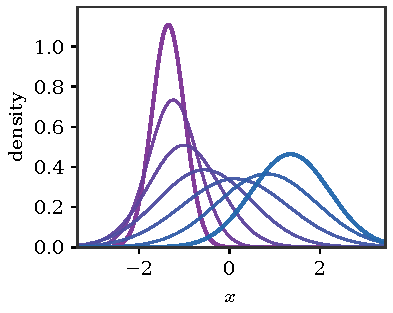
\includegraphics[width=.32\linewidth]{figures/monge-gaussian-fr-mean-geodesic/densities-fr.pdf} \\[-.1em]
\small parameter geodesics &
\small $\Wass_2$ interpolation &
\small Fisher--Rao interpolation
\end{tabular}
\caption{\emph{Wasserstein and Fisher--Rao geodesics in the one-dimensional Gaussian family.} Both interpolations share red and blue endpoint colors. The Wasserstein curves interpolate directly between them, whereas the Fisher--Rao curves pass through green at mid-time; the same palettes identify both geodesics in the left parameter-space panel. The two density panels use the same endpoint Gaussians and time samples, but the Fisher--Rao path expands the standard deviation along its hyperbolic arc before returning to the target scale.}
\label{fig:monge-gaussian-fr-mean-geodesic}
\end{figure}

\paragraph{Multivariate Gaussians.}
\index{Gaussian!measure}% strictindex

As in the scalar case, a natural approach is to seek the optimal transport map within the class of affine maps. If
\eql{\label{eq-gauss-pf}
	\al=\Gaussian(\mean_\al,\cov_\al),
	\qquad
	\be=\Gaussian(\mean_\be,\cov_\be),
	\qquad
	\T(x)=\mean_\be+A(x-\mean_\al),
}
then $\T$ is the gradient of the convex quadratic potential $\phi(x)=\dotp{\mean_\be}{x}+\dotp{A(x-\mean_\al)}{x-\mean_\al}/2$ if and only if $A$ is symmetric positive semidefinite.
\index{quadratic!potential}% strictindex

\begin{prop}[Affine push-forward of Gaussians]\label{prop-gaussian-affine-push-forward}
\index{push-forward}% strictindex
\index{Gaussian!push-forward}% strictindex
	One has $\T_\sharp\al=\be$ if and only if
	\eql{\label{eq-gauss-covariance-pushforward}
		A\cov_\al A^\top=\cov_\be.
	}
\end{prop}
\begin{proof}
	An affine function maps a Gaussian to a Gaussian, so the law of $\T(X)$ is determined by its mean and covariance. If $X\sim\al$ and $Y=\T(X)$, then
	\(\EE(Y)=\mean_\be+A\EE(X-\mean_\al)=\mean_\be\),
	and
	\[
		\EE((Y-\mean_\be)(Y-\mean_\be)^\top)
		=
		A\EE((X-\mean_\al)(X-\mean_\al)^\top)A^\top
		=
		A\cov_\al A^\top.
	\]
	Thus $A\cov_\al A^\top=\cov_\be$ is necessary and sufficient for $Y$ to have the same mean and covariance as $\be$; since both laws are Gaussian, this is equivalent to equality in distribution.
\end{proof}

The covariance equation is quadratic in $A$. Under the symmetry constraint imposed by Brenier's theorem, it becomes $A\cov_\al A=\cov_\be$. The covariance part of the resulting cost is a matrix metric.
\index{Brenier!theorem}% strictindex

\begin{defn}[Bures metric]\label{def-bures-metric}
\index{Bures!metric}% strictindex
\index{positive!semidefinite matrix}% strictindex
	For positive semidefinite covariance matrices $\Sigma$ and $\Lambda$, the Bures metric is
	\eql{\label{eq-bures-defn}
		\Bb(\Sigma,\Lambda)^2
		\eqdef
		\tr\pa{\Sigma+\Lambda-2(\Sigma^{1/2}\Lambda\Sigma^{1/2})^{1/2}}.
	}
\end{defn}
The next proposition solves the covariance equation and shows that this metric is exactly the covariance contribution to Gaussian $\Wass_2$.

\begin{prop}[Gaussian $\Wass_2$ formula and Bures covariance term]\label{prop-gaussian-w2-bures}
\index{covariance!term}% strictindex
\index{Bures!covariance}% strictindex
	Assume that $\cov_\al$ and $\cov_\be$ are positive definite. The covariance equation and its unique symmetric positive-definite solution are
	\eql{\label{eq-bures-map}
		A\cov_\al A=\cov_\be,\quad A\succ0,
		\qquad\Longleftrightarrow\qquad
		A=
		\cov_\al^{-1/2}
		\pa{\cov_\al^{1/2}\cov_\be\cov_\al^{1/2}}^{1/2}
		\cov_\al^{-1/2}.
	}
	The affine map $\T(x)=\mean_\be+A(x-\mean_\al)$ is the optimal quadratic-cost transport from $\Gaussian(\mean_\al,\cov_\al)$ to $\Gaussian(\mean_\be,\cov_\be)$, and
\index{affine!map}% strictindex
\index{quadratic!cost}% strictindex
	\eql{\label{eq-dist-gauss}
		\Wass_2(\al,\be)^2
		=
		\norm{\mean_\al-\mean_\be}^2+\Bb(\cov_\al,\cov_\be)^2,
	}
	where $\Bb$ is the Bures metric of Definition~\ref{def-bures-metric}.
\index{Bures!metric}% strictindex
\end{prop}
\begin{proof}
	Multiplying $A\cov_\al A=\cov_\be$ on the left and right by $\cov_\al^{1/2}$ gives
	$(\cov_\al^{1/2}A\cov_\al^{1/2})^2
	=\cov_\al^{1/2}\cov_\be\cov_\al^{1/2}$.
	Since $A$ is symmetric positive, $\cov_\al^{1/2}A\cov_\al^{1/2}$ is symmetric positive and is therefore the unique positive square root of the right-hand side. Conversely, the matrix in~\eqref{eq-bures-map} is symmetric positive and satisfies the covariance equation.

	By Proposition~\ref{prop-gaussian-affine-push-forward}, this affine map pushes $\al$ to $\be$. It is the gradient of a convex quadratic potential, so Brenier's theorem implies optimality. If $X\sim\al$, then
\index{affine!map}% strictindex
\index{Brenier!theorem}% strictindex
\index{quadratic!potential}% strictindex
\index{push-forward}% strictindex
	\begin{align*}
		\EE\norm{X-\T(X)}^2
		&=
		\norm{\mean_\al-\mean_\be}^2
		+
		\EE\norm{(\Id-A)(X-\mean_\al)}^2 \\
		&=
		\norm{\mean_\al-\mean_\be}^2
		+
		\tr((\Id-A)\cov_\al(\Id-A)^\top) \\
		&=
		\norm{\mean_\al-\mean_\be}^2
		+
		\tr(\cov_\al)+\tr(A\cov_\al A)-2\tr(A\cov_\al) \\
		&=
		\norm{\mean_\al-\mean_\be}^2
		+
		\tr(\cov_\al)+\tr(\cov_\be)
		-2\tr((\cov_\al^{1/2}\cov_\be\cov_\al^{1/2})^{1/2}),
	\end{align*}
	which is the desired expression. The formula for singular covariance matrices follows by adding $\eta\Id$ and letting $\eta\downarrow0$.
\index{covariance!matrix}% strictindex
\end{proof}

\begin{rem}[Common-generator elliptical laws]\label{rem-elliptical-bures}
\index{elliptical law}% strictindex
\index{radial generator}% strictindex
\index{elliptically contoured distribution}% strictindex
\index{Bures!metric}% strictindex
	The Gaussian formula has a useful, but deliberately limited, extension beyond Gaussian tails. Fix an absolutely continuous, centered, radial probability measure $\rho$ on $\RR^d$ with covariance $\Id$. For positive definite matrices $\cov_\al,\cov_\be$, define two elliptically contoured laws with this same radial generator by
	\[
		\al=(z\mapsto \mean_\al+\cov_\al^{1/2}z)_\sharp\rho,
		\qquad
		\be=(z\mapsto \mean_\be+\cov_\be^{1/2}z)_\sharp\rho.
	\]
	For this pair, the same Brenier matrix~\eqref{eq-bures-map} gives the optimal map $\T(x)=\mean_\be+A(x-\mean_\al)$, and the same formula~\eqref{eq-dist-gauss} holds. Indeed, if $X=\mean_\al+\cov_\al^{1/2}Z$ with $Z\sim\rho$, then $A\cov_\al A=\cov_\be$, hence $A\cov_\al^{1/2}=\cov_\be^{1/2}Q$ for some orthogonal matrix $Q$. Since $\rho$ is radial, $QZ$ has the same law as $Z$, so $\T_\sharp\al=\be$. Since $A$ is symmetric positive definite, $\T$ is the gradient of a convex quadratic potential and Brenier's theorem gives optimality. Finally, because $\rho$ is centered with covariance $\Id$, the transport cost depends only on the means and covariance matrices and gives the Bures expression. The common-generator assumption is the point: for two elliptical laws with different radial profiles, one must also transport the radial variable, and the covariance/Bures term is no longer the full transport cost.
\end{rem}

The covariance term $\Bb$ is the Bures--Wasserstein metric on positive semidefinite matrices~\cite{bures1969extension,gelbrich1990formula,bhatia2018bures}. It separates the Euclidean displacement of the mean from the intrinsic transport geometry of covariance ellipsoids.
\begin{rem}[The $2\times2$ covariance cone]\label{rem-2x2-covariance-cone}
\index{Bures!Wasserstein geometry}% strictindex
\index{positive!semidefinite matrix}% strictindex
\index{covariance!term}% strictindex
\index{ice-cream cone}% strictindex
\index{covariance!cone}% strictindex
\index{Lorentz cone}% strictindex
\index{positive!semidefinite cone}% strictindex
\index{Frobenius inner product}% strictindex
	For $2\times2$ covariance matrices, the geometry can be visualized without suppressing any degree of freedom. The following orthonormal coordinates for the Frobenius inner product separate the trace $t$, diagonal anisotropy $u$ and correlation $v$:
	\begin{equation}\label{eq-2x2-covariance-cone}
		\begin{gathered}
			\Sigma=\begin{pmatrix}a&c\\c&b\end{pmatrix}
			\quad\longleftrightarrow\quad
			(t,u,v)=\frac{1}{\sqrt2}(a+b,a-b,2c),
			\qquad
			\Sigma=\frac{1}{\sqrt2}
			\begin{pmatrix}t+u&v\\v&t-u\end{pmatrix},
			\\
			2\det(\Sigma)=t^2-u^2-v^2,
			\qquad
			\mathbb S_+^2
			\quad\longleftrightarrow\quad
			\mathcal K_3
			\eqdef
			\left\{(t,u,v)\in\RR^3:t\geq\sqrt{u^2+v^2}\right\}.
		\end{gathered}
	\end{equation}
	Thus $\mathbb S_+^2$ is the three-dimensional Lorentz, or ice-cream, cone: its apex represents the zero matrix, its nonzero boundary represents rank-one covariances, and its interior represents positive definite covariances. This identification describes the set of admissible matrices, not its Bures geometry. In particular, the Bures distance is not the ambient Euclidean distance of $\RR^3$.

	Figure~\ref{fig:monge-gaussian-w2-geodesic-2d} makes this distinction visible. The first two panels show two Bures--Wasserstein interpolations through covariance ellipses, and the right panel places the same paths in $\mathcal K_3$. Their colored curves remain inside the cone but generally bend away from the faint gray Euclidean chords, because they are geodesics for the Bures metric rather than for the ambient Frobenius metric.
\end{rem}

\begin{figure}[htbp]
\centering
\setlength{\tabcolsep}{2pt}
\begin{tabular}{@{}ccc@{}}
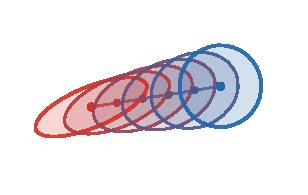
\includegraphics[width=.30\linewidth]{figures/monge-gaussian-w2-geodesic/ellipses-anisotropic-to-isotropic.pdf} &
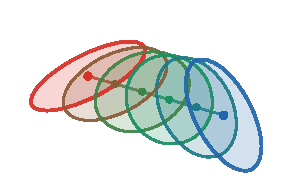
\includegraphics[width=.30\linewidth]{figures/monge-gaussian-w2-geodesic/ellipses-rotated-anisotropic.pdf} &
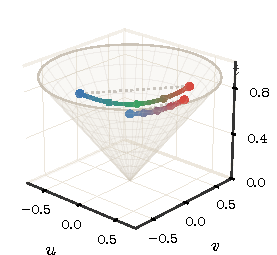
\includegraphics[width=.30\linewidth]{figures/monge-gaussian-w2-geodesic/cone-2d.pdf} \\[-.1em]
\small anisotropic to isotropic &
\small rotated anisotropies &
\small covariance cone
\end{tabular}
\caption{\emph{Two-dimensional Gaussian $\Wass_2$ geodesics.} Means move linearly, while covariance ellipses follow the Bures--Wasserstein interpolation. The left path uses a direct red-to-blue palette; the middle path shares the same endpoint colors but passes through green. The right panel displays these same two palettes along the corresponding covariance paths in the $2\times2$ positive-semidefinite cone, with $u$ and $v$ horizontal and $t$ vertical; faint gray chords show the ambient Euclidean segments for comparison.}
\label{fig:monge-gaussian-w2-geodesic-2d}
\end{figure}



\paragraph{Alternate formulation of the Bures metric.}
Beyond its Gaussian origin, the Bures metric can be recovered from two simpler ambient geometries. It is induced either by $\Wass_2$ after retaining only second moments, or by the Frobenius norm after retaining only the covariance product $AA^\top$.

The first interpretation is distribution-free: it identifies all probability measures with the same second-moment matrix.

\begin{prop}[Bures metric as a second-moment quotient]\label{prop-bures-second-moment-lift}
\index{second-moment quotient}% strictindex
\index{raw second moment}% strictindex
\index{Bures!metric}% strictindex
\index{second moment}% strictindex
\index{positive!semidefinite matrix}% strictindex
	For $\al\in\Pp_2(\RR^d)$, set its raw second-moment matrix to be
	\[
		\Phi_2(\al)\eqdef \int_{\RR^d} uu^\top \d\al(u)\in\mathbb S_+^d.
	\]
	For $\Sigma,\Lambda\in\mathbb S_+^d$,
	\[
		\min_{\Phi_2(\al)=\Sigma,\ \Phi_2(\be)=\Lambda}
		\Wass_2(\al,\be)^2
		=
		\Bb(\Sigma,\Lambda)^2.
	\]
	In other words, the Bures metric is the Wasserstein quotient distance induced on positive semidefinite matrices by identifying all probability measures with the same raw second-moment matrix.
\index{Bures!metric}% strictindex
\end{prop}
\begin{proof}
	Assume first that $\Sigma$ and $\Lambda$ are positive definite. Fix two admissible laws $\al,\be$ and an arbitrary coupling $\pi$ between them, and write
	$K\eqdef\int_{\RR^d\times\RR^d}uv^\top\d\pi(u,v)$. Then
	$\int\norm{u-v}^2\d\pi(u,v)
	=\tr(\Sigma)+\tr(\Lambda)-2\tr(K)$.
	The block second-moment matrix
	\[
		\int
		\begin{pmatrix}u\\ v\end{pmatrix}
		\begin{pmatrix}u\\ v\end{pmatrix}^{\!\top}
		\d\pi(u,v)
		=
		\begin{pmatrix}
			\Sigma & K\\
			K^\top & \Lambda
		\end{pmatrix}
	\]
	is positive semidefinite. The Schur complement gives
	$R\eqdef\Sigma^{-1/2}K\Lambda^{-1/2}$ with $RR^\top\preceq\Id$, so
	$K=\Sigma^{1/2}R\Lambda^{1/2}$ with $\norm{R}_{\mathrm{op}}\leq1$. By duality between the nuclear and operator norms,
	\[
		\tr(K)
		\leq
		\sup_{\norm{R}_{\mathrm{op}}\leq1}\tr(\Sigma^{1/2}R\Lambda^{1/2})
		=
		\norm{\Lambda^{1/2}\Sigma^{1/2}}_*
		=
		\tr\pa{(\Sigma^{1/2}\Lambda\Sigma^{1/2})^{1/2}}.
	\]
	For singular matrices, fix $\eta>0$. Adding $\eta\Id$ to the two diagonal blocks preserves block positivity, so the same Schur-complement argument gives
	\[
		\tr(K)
		\leq
		\tr\pa{((\Sigma+\eta\Id)^{1/2}(\Lambda+\eta\Id)(\Sigma+\eta\Id)^{1/2})^{1/2}}.
	\]
	Letting $\eta\downarrow0$ and using continuity of the matrix square root gives the same trace bound with $\Sigma,\Lambda$. Hence every admissible coupling has cost at least $\Bb(\Sigma,\Lambda)^2$.

	Conversely, choose the centered Gaussian laws $\Gaussian(0,\Sigma)$ and $\Gaussian(0,\Lambda)$. They satisfy the two second-moment constraints, and Proposition~\ref{prop-gaussian-w2-bures} gives
	$\Wass_2(\Gaussian(0,\Sigma),\Gaussian(0,\Lambda))^2
	=\Bb(\Sigma,\Lambda)^2$, again by continuity in the singular case. This admissible pair attains the lower bound, proving the claim.
\end{proof}

The second interpretation is purely matrix-based: it identifies all matrix factors with the same covariance product.

\begin{prop}[Bures metric as a Procrustes metric]\label{prop-bures-procrustes}
\index{Bures!Procrustes representation}% strictindex
\index{Procrustes!Bures metric}% strictindex
	Let $\Sigma,\Lambda\in\mathbb S_+^d$, let $d'\geq d$, and fix any
	$A_0,B_0\in\RR^{d\times d'}$ such that
	$A_0A_0^\top=\Sigma$ and $B_0B_0^\top=\Lambda$. Then
		\begin{equation}\label{eq-bures-procrustes}
			\Bb(\Sigma,\Lambda)^2
			=
			\min_{\substack{A,B\in\RR^{d\times d'}\\
				AA^\top=\Sigma,\;BB^\top=\Lambda}}
			\norm{A-B}_{\mathrm F}^2
			=
			\min_{R\in\mathrm O(d')}\norm{A_0-B_0R}_{\mathrm F}^2.
		\end{equation}
	For $d'=d$, one may in particular take $A_0=\Sigma^{1/2}$ and
	$B_0=\Lambda^{1/2}$; the second minimum is then over $\mathrm O(d)$.
\end{prop}
\begin{proof}
	Two matrices in $\RR^{d\times d'}$ have the same row-Gram matrix if and
	only if they differ by right multiplication by an orthogonal matrix. Indeed,
	equality of the Gram matrices makes the linear map sending each row of one
	matrix to the corresponding row of the other well defined and isometric on
	their row spans; this isometry extends to an element of $\mathrm O(d')$.
	Therefore every admissible pair has the form $A=A_0U$ and $B=B_0V$ for
	some $U,V\in\mathrm O(d')$. Right invariance of the Frobenius norm gives
	\[
		\min_{U,V\in\mathrm O(d')}\norm{A_0U-B_0V}_{\mathrm F}^2
		=
		\min_{R\in\mathrm O(d')}\norm{A_0-B_0R}_{\mathrm F}^2,
	\]
	where one may take $R=VU^\top$. Thus the two factor minima in
	\eqref{eq-bures-procrustes} coincide and are independent of the chosen
	representatives $A_0,B_0$.

	Expanding the last objective and applying the orthogonal Procrustes formula,
	which follows directly from a singular-value decomposition, yields
	\[
		\min_{R\in\mathrm O(d')}\norm{A_0-B_0R}_{\mathrm F}^2
		=
		\tr(\Sigma)+\tr(\Lambda)-2\norm{A_0^\top B_0}_*.
	\]
	Moreover,
	$(A_0^\top B_0)^\top(A_0^\top B_0)=B_0^\top\Sigma B_0$, whose nonzero
	eigenvalues are those of
		$\Sigma^{1/2}B_0B_0^\top\Sigma^{1/2}
		=\Sigma^{1/2}\Lambda\Sigma^{1/2}$. Consequently,
		$\norm{A_0^\top B_0}_*
		=\tr((\Sigma^{1/2}\Lambda\Sigma^{1/2})^{1/2})$.
	Definition~\ref{def-bures-metric} now identifies the resulting value with
	$\Bb(\Sigma,\Lambda)^2$.
\end{proof}

Thus the map $A\mapsto AA^\top$ identifies $\mathbb S_+^d$ with the orbit
space $\RR^{d\times d'}/\mathrm O(d')$, and $\Bb$ is the quotient distance
induced by the Frobenius metric. This is the matrix counterpart of the quotient
transport geometries developed in
Section~\ref{sec-quotient-wasserstein-procrustes}.

These two representations make the metric and convexity properties of $\Bb$ transparent.

\begin{prop}[Metric and convexity properties of the Bures term]\label{prop-bures-metric-convex}
\index{Bures!metric}% strictindex
	The function $\Bb$ is a distance on positive semidefinite covariance matrices. Moreover, $\Bb^2$ is jointly convex: for $t\in[0,1]$,
\index{covariance!matrix}% strictindex
	\[
		\Bb^2((1-t)\Sigma_0+t\Sigma_1,(1-t)\Lambda_0+t\Lambda_1)
		\leq
		(1-t)\Bb^2(\Sigma_0,\Lambda_0)+t\Bb^2(\Sigma_1,\Lambda_1).
	\]
\end{prop}
\begin{proof}
	The free-factor formula in Proposition~\ref{prop-bures-procrustes} is
	symmetric and nonnegative. Since its minima are attained, it vanishes if and
	only if two factors coincide, which is equivalent to $\Sigma=\Lambda$.
	For the triangle inequality, use the square-factor specialization and let
	$Q_1,Q_2$ be optimal orthogonal alignments for $(\Sigma,\Lambda)$ and
	$(\Lambda,\Gamma)$, respectively.
	Since $Q_2Q_1$ is admissible for $(\Sigma,\Gamma)$,
\index{triangle inequality}% strictindex
	\[
		\Bb(\Sigma,\Gamma)
		\leq
		\norm{\Sigma^{1/2}-\Gamma^{1/2}Q_2Q_1}_{\mathrm F}
		\leq
		\norm{\Sigma^{1/2}-\Lambda^{1/2}Q_1}_{\mathrm F}
		+
		\norm{\Lambda^{1/2}-\Gamma^{1/2}Q_2}_{\mathrm F}
		=
		\Bb(\Sigma,\Lambda)+\Bb(\Lambda,\Gamma).
	\]

	For convexity, use the free-factor formula in
	Proposition~\ref{prop-bures-procrustes}. For $i\in\{0,1\}$, choose optimal
	square factors $(U_i,V_i)$ for $(\Sigma_i,\Lambda_i)$ and define the block
	factors
	\[
		U_t=[\sqrt{1-t}\,U_0,\sqrt t\,U_1],
		\qquad
		V_t=[\sqrt{1-t}\,V_0,\sqrt t\,V_1].
	\]
	Set $\Sigma_t=(1-t)\Sigma_0+t\Sigma_1$ and
	$\Lambda_t=(1-t)\Lambda_0+t\Lambda_1$. Then
	$U_tU_t^\top=\Sigma_t$ and $V_tV_t^\top=\Lambda_t$. Applying the
		free-factor formula with $2d$ columns gives
		\[
			\Bb^2(\Sigma_t,\Lambda_t)
			\leq\norm{U_t-V_t}_{\mathrm F}^2
			=(1-t)\norm{U_0-V_0}_{\mathrm F}^2+t\norm{U_1-V_1}_{\mathrm F}^2
			=(1-t)\Bb^2(\Sigma_0,\Lambda_0)+t\Bb^2(\Sigma_1,\Lambda_1),
		\]
	which proves joint convexity.
\end{proof}

\begin{rem}[Diagonal covariances and Hellinger geometry]
\index{covariance!diagonal}% strictindex
\index{Hellinger!geometry}% strictindex
	If $\cov_\al=\diag(r_i)_i$ and $\cov_\be=\diag(s_i)_i$ are diagonal, the Bures metric reduces to the Euclidean distance between square roots,
\index{Bures!metric}% strictindex
	$\Bb(\cov_\al,\cov_\be)=\norm{\sqrt r-\sqrt s}_2$.
	This is the finite-dimensional Hellinger geometry on the nonnegative covariance coordinates: variances are compared after the amplitude change of variables $r_i\mapsto\sqrt{r_i}$.
\index{change of variables formula}% strictindex
\end{rem}

\paragraph{Comparison with the Fisher--Rao metric for zero-mean Gaussians.}
\index{affine-invariant metric}% strictindex
\index{rank-deficient covariance}% strictindex
\index{Fisher-Rao@Fisher--Rao metric}% strictindex
\index{Kullback-Leibler@Kullback--Leibler!divergence}% strictindex
\index{Bures!metric}% strictindex
The Bures metric is the covariance geometry induced by quadratic optimal transport. A different, information-geometric metric is obtained by expanding the Kullback--Leibler divergence between centered Gaussians. For $\Sigma,\Sigma'\in\mathbb S_{++}^d$, write
\[
	\KL(\Sigma\mid\Sigma')
	\eqdef
	\KL\big(\Gaussian(0,\Sigma)\mid\Gaussian(0,\Sigma')\big)
	=
	\frac12\left(
	\tr((\Sigma')^{-1}\Sigma)-d-\log\det((\Sigma')^{-1}\Sigma)
	\right).
\]
If $D=D^\top$ and $\Sigma+\varepsilon D$ remains positive definite, then
\[
	\KL(\Sigma+\varepsilon D\mid\Sigma)
	=
	\frac{\varepsilon^2}{2}\langle Q_\Sigma(D),D\rangle_F+o(\varepsilon^2),
	\qquad
	Q_\Sigma(D)=\frac12\Sigma^{-1}D\Sigma^{-1},
\]
where $\langle A,B\rangle_F=\tr(A^\top B)$ is the Frobenius pairing. Thus the local quadratic form is
\[
	g_\Sigma(D,E)=\frac12\tr(\Sigma^{-1}D\Sigma^{-1}E).
\]
With this normalization, the Fisher--Rao, or affine-invariant, geodesic distance on $\mathbb S_{++}^d$ is
\index{Fisher-Rao@Fisher--Rao metric}% strictindex
\[
	d_{\mathrm{FR}}(\Sigma,\Sigma')^2
	=
	\frac12
	\norm{\log(\Sigma^{-1/2}\Sigma'\Sigma^{-1/2})}_F^2,
\]
where $\log$ denotes the principal matrix logarithm, and the corresponding geodesic is
\[
	\Sigma_t^{\mathrm{FR}}
	=
	\Sigma^{1/2}
	\left(\Sigma^{-1/2}\Sigma'\Sigma^{-1/2}\right)^t
	\Sigma^{1/2}.
\]
The contrast with Bures is especially visible near the boundary of the covariance cone. For example, $\Bb^2(\Sigma,0)=\tr(\Sigma)$, and more generally the Bures formula extends continuously to $\mathbb S_+^d$; rank-deficient covariance matrices are therefore at finite distance and the closed cone is part of the metric completion. Fisher--Rao is different. If an eigenvalue of $\Sigma^{-1/2}\Sigma'\Sigma^{-1/2}$ tends to zero, then the corresponding logarithm diverges in $d_{\mathrm{FR}}$. Hence the boundary, made of degenerate covariance matrices and representing infinitely anisotropic Gaussian limits on fixed-trace sections, is at infinite distance.

In the coordinates~\eqref{eq-2x2-covariance-cone}, write $z=(t,u,v)$ and $z'=(t',u',v')$, and set
\[
	\Delta_z=t^2-u^2-v^2,\qquad
	\langle z,z'\rangle_{\mathrm E}=tt'+uu'+vv',
	\qquad
	\langle z,z'\rangle_{\mathrm L}=tt'-uu'-vv'.
\]
Then the two distances admit the side-by-side expressions
\begin{align}
	\Bb(\Sigma,\Sigma')^2
	&=
	\sqrt2(t+t')
	-2\sqrt{\langle z,z'\rangle_{\mathrm E}
	+\sqrt{\Delta_z\Delta_{z'}}},
	\label{eq-2x2-bures-cone-distance}\\
	d_{\mathrm{FR}}(\Sigma,\Sigma')^2
	&=
	\frac12\left((\log\lambda_+)^2+(\log\lambda_-)^2\right),
	\qquad
	\lambda_\pm
	=
	\frac{\langle z,z'\rangle_{\mathrm L}
	\pm\sqrt{\langle z,z'\rangle_{\mathrm L}^2-\Delta_z\Delta_{z'}}}
	{\Delta_z},
	\label{eq-2x2-fr-cone-distance}
\end{align}
where the Fisher--Rao formula requires $\Delta_z,\Delta_{z'}>0$ and $\lambda_\pm$ are the eigenvalues of $\Sigma^{-1}\Sigma'$. Figure~\ref{fig:monge-gaussian-fr-vs-bures-cone} shows this contrast in the $2\times2$ ice-cream cone: the Bures path reaches a rank-one covariance, while the Fisher--Rao path is drawn only to a small positive-definite regularization of the same rank-one limit.
\index{Fisher-Rao@Fisher--Rao metric}% strictindex

\begin{figure}[htbp]
\centering
\setlength{\tabcolsep}{3pt}
\begin{tabular}{@{}cc@{}}
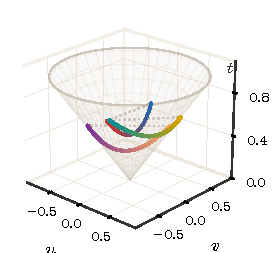
\includegraphics[width=.38\linewidth]{figures/monge-gaussian-fr-vs-bures-cone/bures-cone.pdf} &
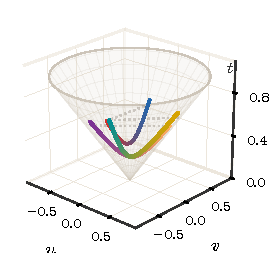
\includegraphics[width=.38\linewidth]{figures/monge-gaussian-fr-vs-bures-cone/fisher-rao-cone.pdf} \\[-.1em]
\small Bures--Wasserstein &
\small Fisher--Rao
\end{tabular}
\caption{\emph{Bures--Wasserstein and Fisher--Rao covariance geodesics in the $2\times2$ positive-semidefinite cone.} Both panels use the coordinates $u=(a-b)/\sqrt2$, $v=\sqrt2c$, $t=(a+b)/\sqrt2$ for $\Sigma=\left(\begin{smallmatrix}a&c\\c&b\end{smallmatrix}\right)$. The three trajectories use distinct red-to-blue, orange-to-violet, and teal-to-gold palettes, repeated identically in both panels to identify corresponding endpoints; faint gray chords show the ambient Euclidean segments. The Bures geodesics can reach rank-deficient covariances on the boundary, whereas the Fisher--Rao geodesics are drawn toward small positive-definite regularizations. The omitted boundary endpoints correspond to rank-one limiting covariances, which are not at finite Fisher--Rao distance.}
\label{fig:monge-gaussian-fr-vs-bures-cone}
\end{figure}
